% =====================================================================
% Appendix: iterative reconstruction of the spatial weights matrix
%
% Usage in the main paper (after \appendix):
%     % =====================================================================
% Appendix: iterative reconstruction of the spatial weights matrix
%
% Usage in the main paper (after \appendix):
%     % =====================================================================
% Appendix: iterative reconstruction of the spatial weights matrix
%
% Usage in the main paper (after \appendix):
%     % =====================================================================
% Appendix: iterative reconstruction of the spatial weights matrix
%
% Usage in the main paper (after \appendix):
%     \input{appendix_reconstruction}
% Figures are read from ../simulation/figures/ (set in the preamble with
%     \graphicspath{{../simulation/figures/}}
% or copy the PNG files next to the .tex file).
% Packages used: graphicx, amsmath (both loaded by sn-jnl).
% Figures and tables are produced by simulation/04_iteration_figures.R from the
% results of simulation/01_ ... 06_*.R in the project repository.
% =====================================================================

\section{Iterative reconstruction of the spatial weights matrix}
\label{app:reconstruction}

This appendix describes an extension of the eigenvector spatial filtering (ESF) step that reconstructs a sparser spatial weights matrix from the selected eigenvectors and iterates the selection on the reconstructed graph. We evaluate it in simulation and explain why it is not part of the proposed procedure.

\subsection{The iterative reconstruction}
\label{app:rec-procedure}

Let $A$ be the $n\times n$ binary contiguity matrix of the study region, $Y$ the standardised counts per cell and $Z$ the standardised covariates. The procedure starts from $D^{(0)}=A$ and, at iteration $k$:

\begin{enumerate}
  \item computes the eigendecomposition $D^{(k)} = E\,\Delta\,E^\top$, with $\Delta=\mathrm{diag}(\delta_1,\dots,\delta_n)$, and selects a subset $S$ of eigenvectors with the MI-Lasso estimator, with penalty $\lambda=|z_0|^{-2}$ fixed from the standardised Moran's $I$ of the residuals of $Y$ on $Z$;
  \item reconstructs
  \begin{equation}
    B = E_S\,\Delta_S\,E_S^\top, \qquad b_{ij} = \sum_{s\in S}\delta_s\, e_s(i)\, e_s(j);
    \label{eq:app-B}
  \end{equation}
  \item applies a rounding rule: among the edges of $D^{(k)}$ with $b_{ij}>0$, it keeps those with $b_{ij}\ge\tau^{(k)}$, where $\tau^{(k)}$ is a threshold computed from these values, giving $D^{(k+1)} = D^{(k)}\circ\mathbf{1}\{B\ge\tau^{(k)}\}$;
  \item accepts $D^{(k+1)}$ if the post-Lasso residuals obtained with its eigenvectors show no spatial correlation (Moran's $I$ with $A$, level $0.05$), and stops otherwise or when $D^{(k+1)}=D^{(k)}$.
\end{enumerate}

Because each accepted step removes at least one edge, the procedure stops after at most as many iterations as $A$ has edges. Cells are then ranked by a ranking rule applied to the final graph.

We call \emph{baseline configuration} the procedure with all $n$ eigenvectors as candidates, eigenvalue weights in \eqref{eq:app-B}, the 75\% quantile of the positive $b_{ij}$ as threshold, and cells ranked by harmonic centrality on the final graph. Each variant below changes one element of the baseline.

\paragraph{Rounding rules.}
\emph{None} (all edges kept, $D=A$; no reconstruction);
\emph{quantile $q$} ($\tau$ = $q$-quantile of the positive $b_{ij}$ on the current edges, $q\in\{0.50, 0.75, 0.80, 0.90\}$);
\emph{mixture} (a two-component Gaussian mixture fitted to the positive $b_{ij}$; $\tau$ is the point between the two means where the weighted component densities are equal, and all edges are kept when the Bayesian information criterion selects one component);
\emph{permutation} (30 Freedman--Lane permutations of the residuals of $Y$ on $Z$; for each, the selection and \eqref{eq:app-B} are recomputed on the current graph, and $\tau$ is the 95th percentile of the pooled positive $b_{ij}$).

\paragraph{Ranking rules.}
Let $\hat f = E_S\hat\gamma_S$ be the fitted spatial component (centred), and call a cell \emph{hot} if $\hat f_i>0$ and \emph{cold} otherwise.
\emph{Centrality, whole graph}: harmonic centrality on the final graph, over all cells (baseline).
\emph{Centrality, hot cells}: harmonic centrality computed among hot cells only.
\emph{Largest excess}: hot cells ordered by $\hat f_i$.
\emph{Hot zones first}: connected groups of hot cells ordered by $\sum_{i}\hat f_i$; within a group, cells ordered by harmonic centrality.
Two benchmarks that do not use the graph are also reported: \emph{top counts} (cells ordered by $Y$) and \emph{top residuals} (cells ordered by the residuals of $Y$, or of $\log(Y+1)$, on $Z$).

\subsection{Simulation design}
\label{app:rec-design}

All scenarios use a $1000\times1000$ window divided into a regular grid with queen contiguity. Table~\ref{tab:app-scenarios} lists the scenarios.

\begin{table}[ht]
\centering
\caption{Simulated scenarios.}
\label{tab:app-scenarios}
\begin{tabular}{p{0.16\textwidth}p{0.50\textwidth}p{0.24\textwidth}}
\hline
Scenario & Data-generating process & Target \\
\hline
A: clusters & Three clusters: parents uniform in the window at least 100 units from the border; 500 offspring per parent, uniform in a disc of radius 100; 2000 additional uniform points. No covariate. & Cells inside the three discs \\
B: clusters and covariate & Scenario A plus 3000 points accepted with probability $\exp\{3(b(x)-1)\}$, where $b$ is a Gaussian surface (standard deviation 150) centred at least 300 units from every parent. The model receives $Z=(b,\ \varepsilon)$ at the cell centres, with $\varepsilon\sim N(0,1)$. & Cells inside the three discs, not the covariate area \\
D: barriers & $Y=\rho W Y + Z\beta + e$ on a $20\times20$ grid, with $W$ the row-standardised version of a graph $W^\ast\subset A$ in which a vertical line (one crossing left open) and a horizontal line on the left half remove 85 of the 1482 edges; $Z$ a linear gradient and noise, $\beta=(1,0)$, $\rho\in\{0.5,0.8,0.95\}$. & The 85 removed edges \\
D0: no barriers & As D with $W^\ast=A$. & No edge removed \\
\hline
\end{tabular}
\end{table}

Unless stated otherwise the grid has $20\times20$ cells (cell side 50) and the budget is the top 20 cells (5\%). For scenarios A and B, \emph{precision} is the share of the selected cells inside a true cluster disc. For scenarios D and D0, edges are classified as kept or removed, and we report the area under the ROC curve (AUC) of $b_{ij}$ for separating real from barrier edges, the share of edges kept, and Youden's $J$ = (share of barrier edges removed) + (share of real edges kept) $-\,1$, which is 0 for a classification unrelated to the barriers.

\subsection{Results}
\label{app:rec-results}

\paragraph{Sign of the reconstructed weights.}
Equation~\eqref{eq:app-B} is invariant to the sign of each eigenvector, since $e_s e_s^\top=(-e_s)(-e_s)^\top$. A positive $b_{ij}$ indicates that cells $i$ and $j$ lie on the same side of the selected spatial patterns, whether both have high or both have low counts. Under the baseline configuration, half of the 20 cells ranked highest in scenario B had $\hat f_i<0$, and precision was 0.28 in scenario A and 0.24 in scenario B (Fig.~\ref{fig:app-cold}). Ranking hot cells by $\hat f$ gave 1.00 and 0.96. Figure~\ref{fig:app-example} shows the successive graphs and the selected cells for one simulated map.

\begin{figure}[ht]
\centering
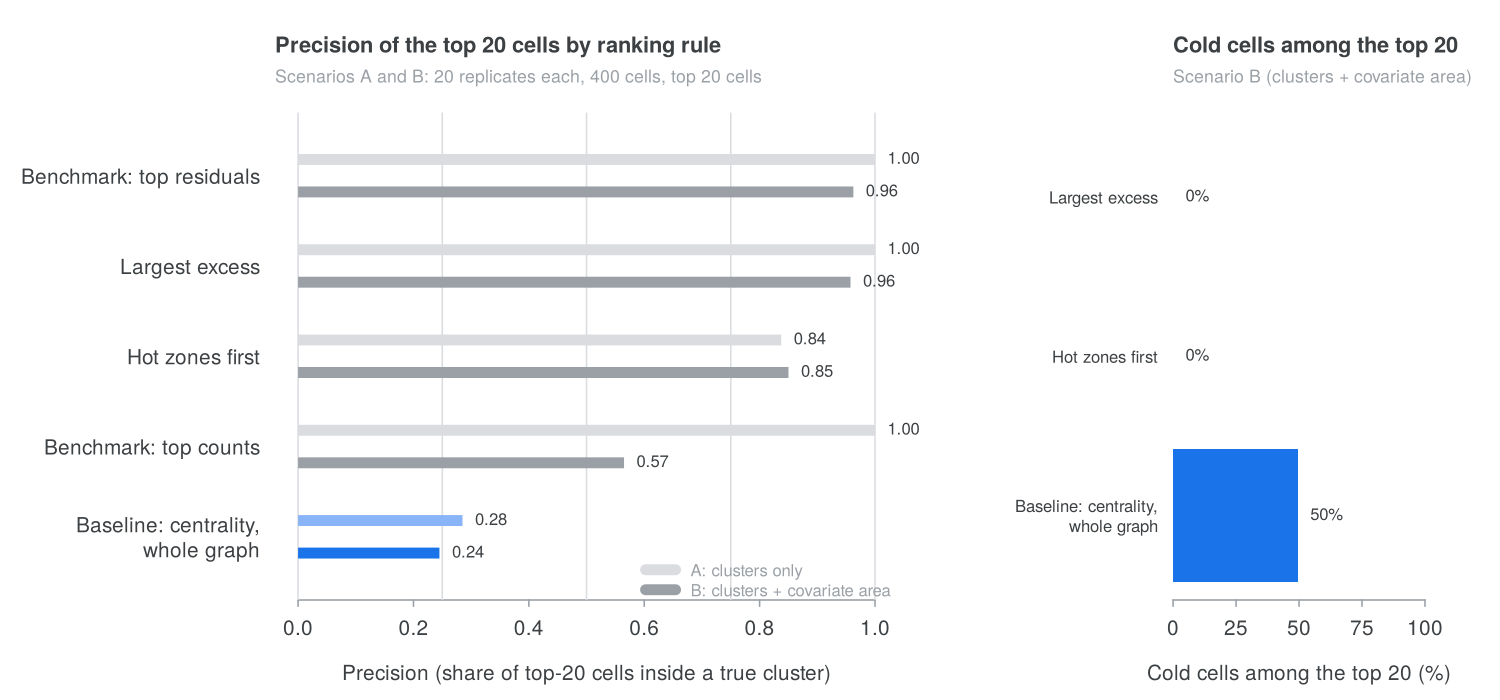
\includegraphics[width=\textwidth]{fig1_cold_zones}
\caption{Precision of the top 20 of 400 cells by ranking rule (scenarios A and B, 20 replicates each) and share of cold cells among them (scenario B). Baseline: harmonic centrality on the final graph.}
\label{fig:app-cold}
\end{figure}

\begin{figure}[ht]
\centering
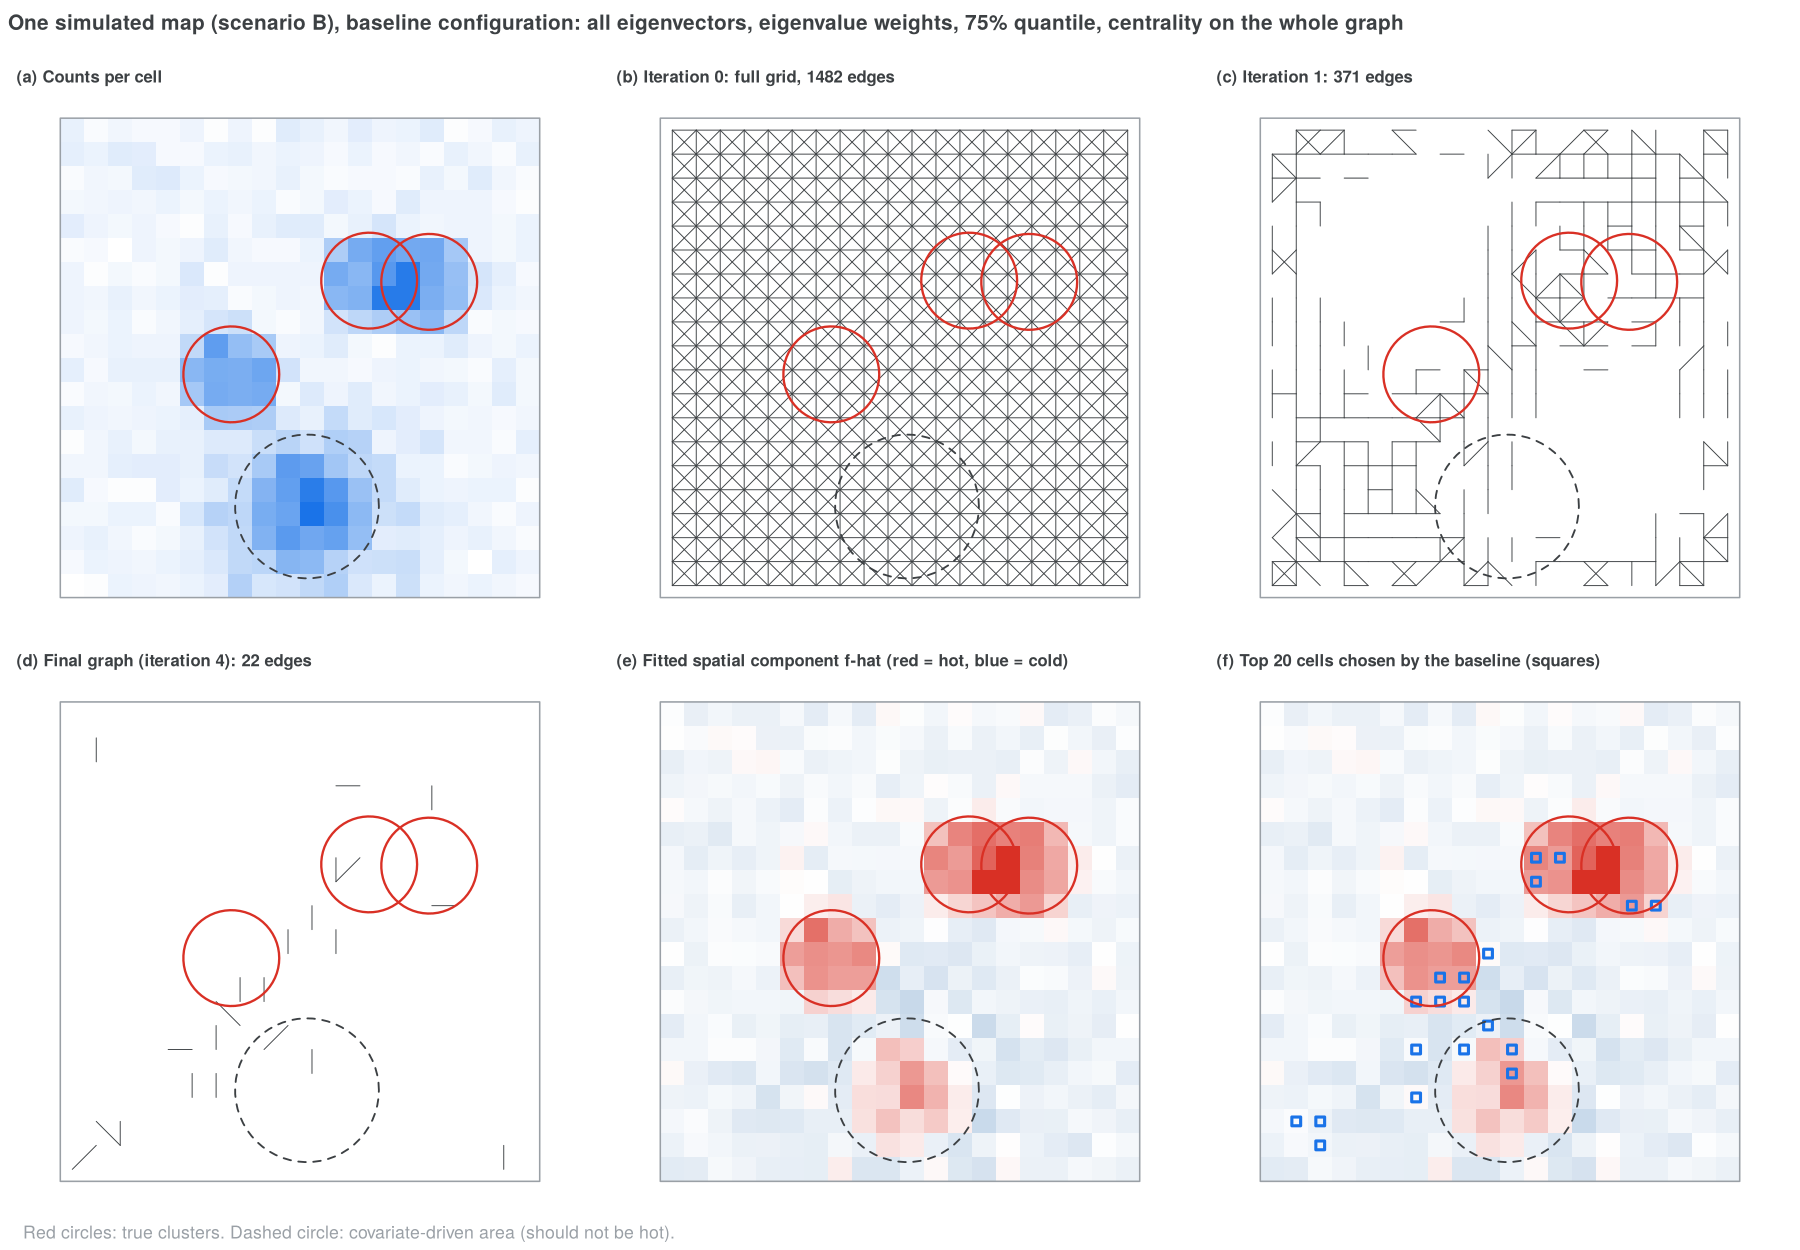
\includegraphics[width=\textwidth]{figS2_example_run}
\caption{One simulated map from scenario B under the baseline configuration. (a) Counts per cell. (b)--(d) Graph at iterations 0, 1 and at the last accepted iteration. (e) Fitted spatial component $\hat f$. (f) Top 20 cells under the baseline ranking. Circles: true clusters; dashed circle: covariate area.}
\label{fig:app-example}
\end{figure}

\paragraph{Effect of rounding and iteration on the selected cells.}
We compared rounding with the 75\% quantile against no rounding over 162 settings of scenario B: grids of $10\times10$, $20\times20$ and $40\times40$ cells, 50, 200 or 500 points per cluster, penalty exponents $a\in\{0.5,1,2\}$ in $\lambda=|z_0|^{-a}$, counts on the original or the $\log(Y+1)$ scale, and three ranking rules (10 replicates per setting). Iteration removed edges in 495 of 1620 runs (31\%); in the remaining runs the first reduced graph was rejected by the Moran test. In the runs where edges were removed, the change in precision was $+0.06$ (95\% CI $0.02$ to $0.10$) for centrality on the whole graph, $-0.01$ ($-0.03$ to $0.01$) for largest excess and $-0.06$ ($-0.11$ to $-0.01$) for hot zones first (Fig.~\ref{fig:app-iteration}).

\begin{figure}[ht]
\centering
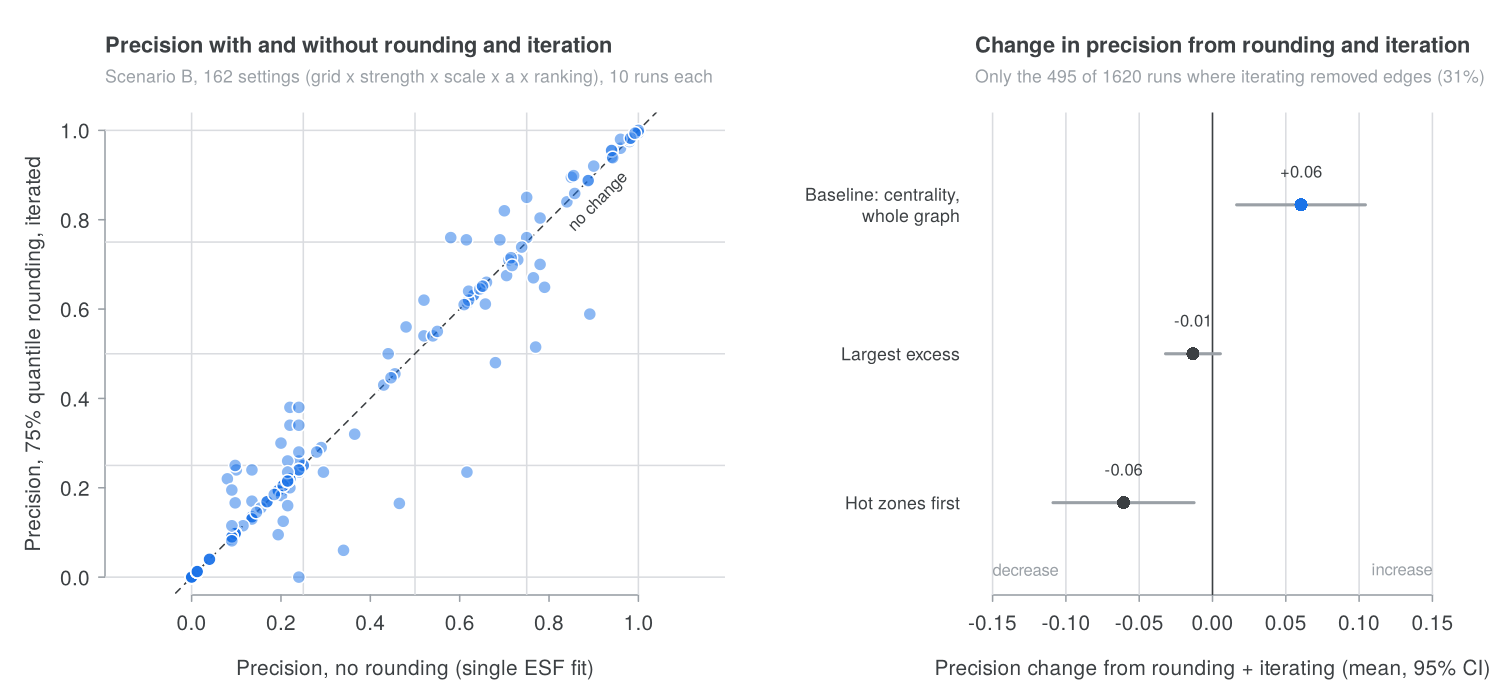
\includegraphics[width=\textwidth]{fig2_iteration_no_effect}
\caption{Left: precision with no rounding against precision with 75\% quantile rounding and iteration; each point is one setting (mean of 10 replicates). Right: change in precision in the runs where iteration removed edges (mean and 95\% confidence interval).}
\label{fig:app-iteration}
\end{figure}

\paragraph{Rounding rules.}
Table~\ref{tab:app-rounding} and Fig.~\ref{fig:app-rounding} compare the seven rounding rules with all other elements fixed at the baseline (scenarios A and B, 20 replicates each; scenarios D and D0, 20 replicates each). With the largest-excess ranking, precision was 1.00 in scenario A and 0.95--0.96 in scenario B for every rule, including no rounding. With hot zones first, the 80\% and 90\% quantiles and the permutation rule gave about 0.10 more than no rounding, and remained below the largest-excess ranking. With the baseline ranking, precision ranged from 0.10 to 0.37. In scenario D0 every rule except the mixture removed between 90\% and 97\% of the edges.

\begin{table}[ht]
\centering
\caption{Precision of the top 20 cells (scenario A / scenario B) by rounding rule and ranking rule, and share of edges kept in scenario D0. Mean of 20 replicates.}
\label{tab:app-rounding}
\small\setlength{\tabcolsep}{4pt}
\begin{tabular}{lcccc}
\hline
Rounding rule & Largest excess & Hot zones first & Centrality, & Edges kept \\
 & & & whole graph & (D0) \\
\hline
None            & 1.00 / 0.95 & 0.85 / 0.76 & 0.13 / 0.10 & 100\% \\
50\% quantile   & 1.00 / 0.95 & 0.81 / 0.71 & 0.32 / 0.37 & 6\% \\
75\% quantile (baseline) & 1.00 / 0.95 & 0.84 / 0.84 & 0.22 / 0.29 & 8\% \\
80\% quantile   & 1.00 / 0.95 & 0.89 / 0.90 & 0.19 / 0.31 & 3\% \\
90\% quantile   & 1.00 / 0.95 & 0.91 / 0.91 & 0.26 / 0.32 & 10\% \\
Mixture         & 1.00 / 0.96 & 0.80 / 0.78 & 0.26 / 0.31 & 76\% \\
Permutation     & 1.00 / 0.95 & 0.90 / 0.91 & 0.23 / 0.37 & 10\% \\
\hline
\end{tabular}
\end{table}

\begin{figure}[ht]
\centering
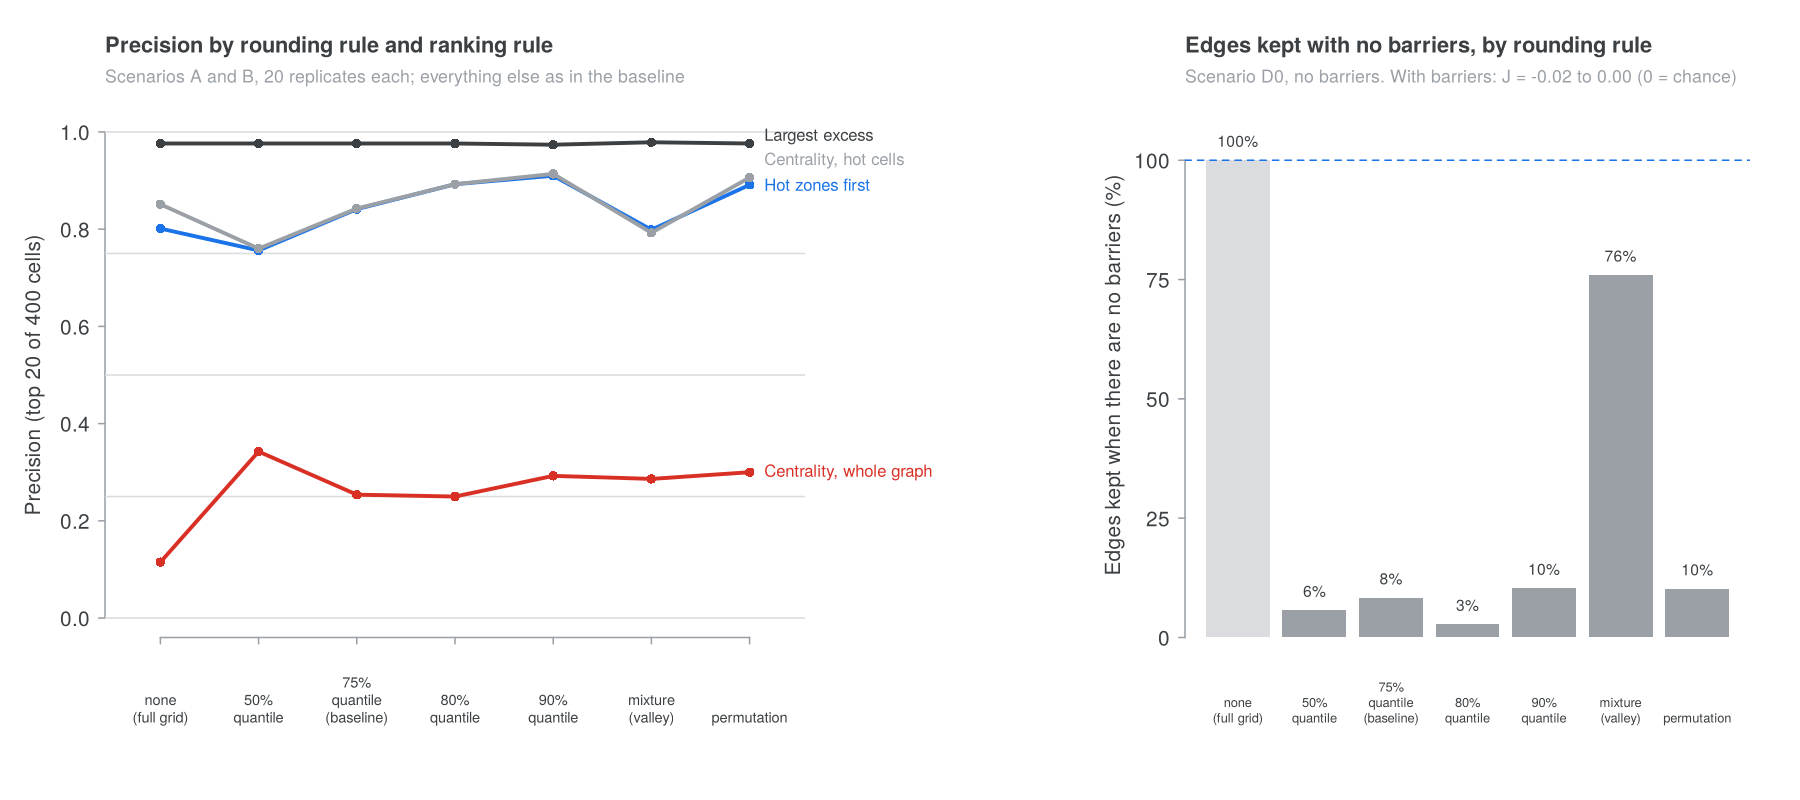
\includegraphics[width=\textwidth]{fig4_rounding_rules}
\caption{Left: precision of the top 20 of 400 cells by rounding rule and ranking rule (scenarios A and B pooled, 20 replicates each). Right: share of edges kept in scenario D0, where no edge should be removed.}
\label{fig:app-rounding}
\end{figure}

\paragraph{Fine grid with weak clusters.}
On a $40\times40$ grid (cell side 25) with 50 or 200 points per cluster, scenario B, budget of 80 cells, 10 replicates, the rankings that use hot cells and connectivity reached, with no rounding, a precision of 0.44--0.48 (50 points) and 0.81--0.89 (200 points), against 0.29 and 0.80 for top residuals on the log scale. Rounding reduced the precision of hot zones first by 0.24 and 0.25 (75\% quantile), 0.18 and 0.17 (90\% quantile) and 0.06 and 0.10 (permutation) (Fig.~\ref{fig:app-finegrid}).

\begin{figure}[ht]
\centering
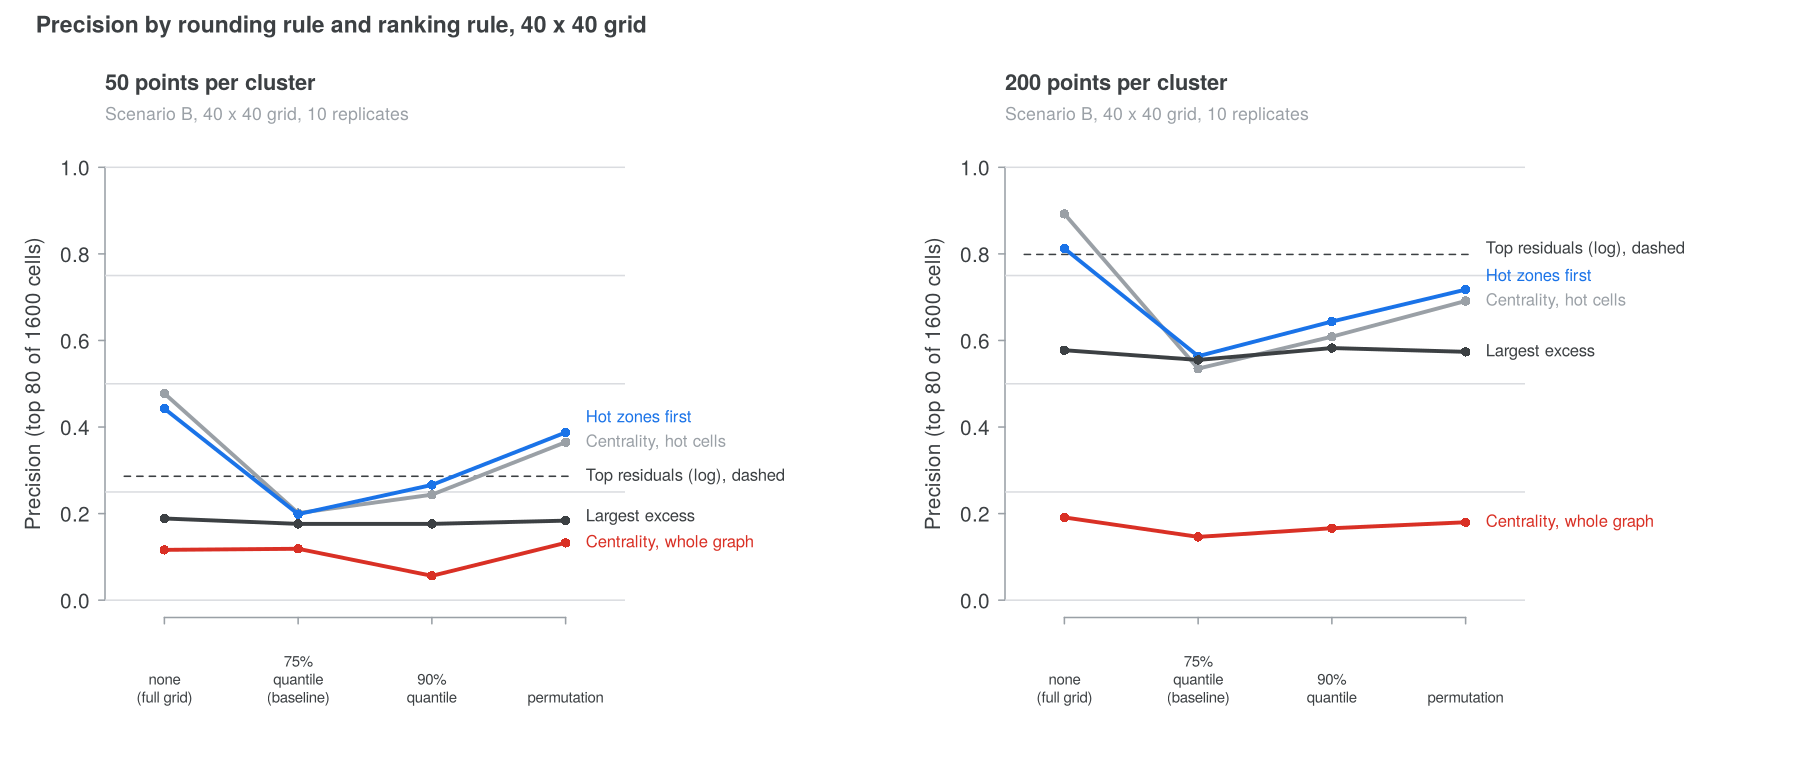
\includegraphics[width=\textwidth]{fig5_fine_grid}
\caption{Precision of the top 80 of 1600 cells by rounding rule and ranking rule on a $40\times40$ grid (scenario B, 10 replicates per panel). Dashed line: top residuals of $\log(Y+1)$ on $Z$.}
\label{fig:app-finegrid}
\end{figure}

\paragraph{Recovery of a known graph.}
In scenario D, the AUC of $b_{ij}$ for separating real from barrier edges was 0.55, 0.55 and 0.45 for $\rho=0.5$, $0.8$ and $0.95$ with eigenvalue weights, and 0.55, 0.53 and 0.61 with squared coefficients $\hat\gamma_s^2$ as weights. The absolute difference between the residuals of neighbouring cells, $|e_i-e_j|$, gave 0.55, 0.65 and 0.96 (Fig.~\ref{fig:app-graph}). After the full procedure, Youden's $J$ ranged from $-0.02$ to $0.00$ across rounding rules. With 130--300 of 400 eigenvectors selected, $B$ differs from $A$ by a small number of patterns with global support, while a barrier is a local discontinuity.

\begin{figure}[ht]
\centering
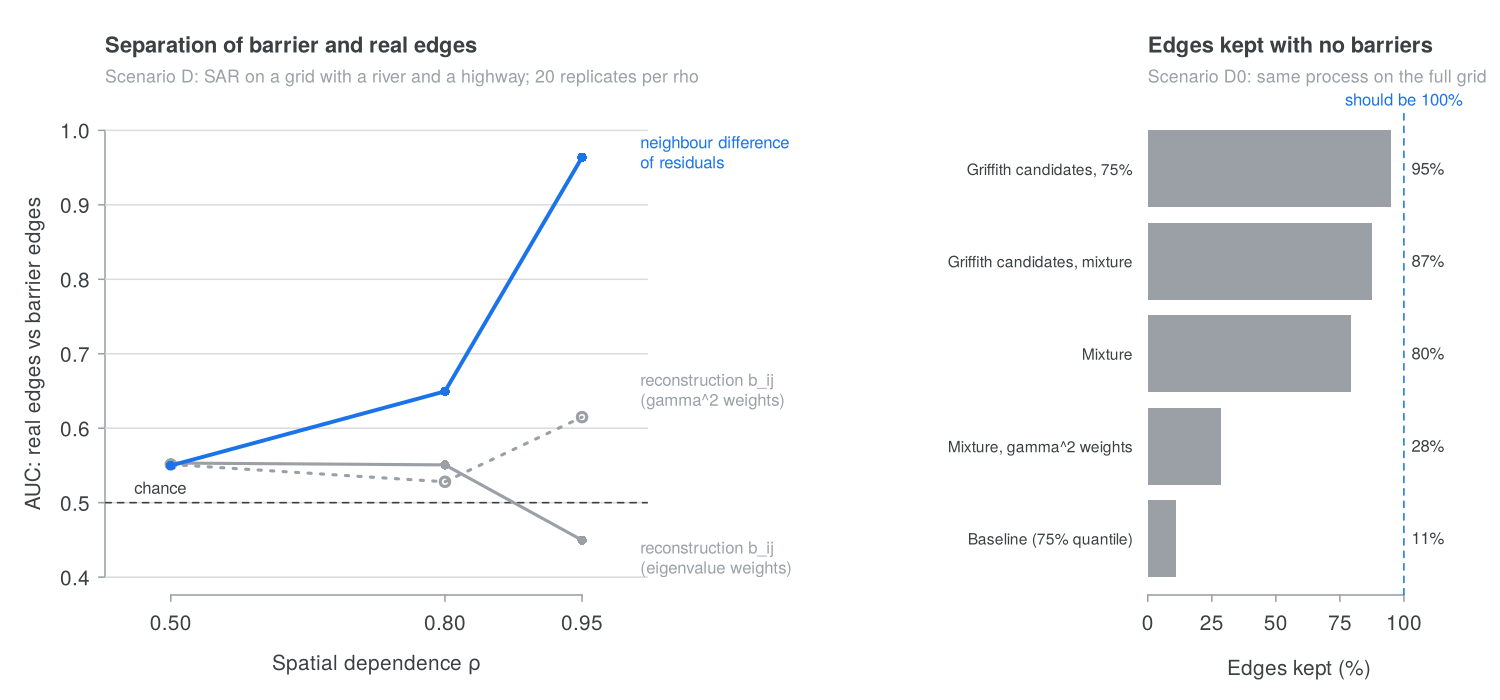
\includegraphics[width=\textwidth]{fig3_latent_graph}
\caption{Left: AUC for separating real edges from barrier edges in scenario D (20 replicates per $\rho$). Right: share of edges kept in scenario D0 by variant of the procedure.}
\label{fig:app-graph}
\end{figure}

\subsection{Conclusion}
\label{app:rec-conclusion}

In these simulations, no rounding rule increased the highest precision obtained without rounding by more than 0.01 (largest excess on the $20\times20$ grid; centrality among hot cells on the $40\times40$ grid). The reconstructed weights did not identify the edges removed by barriers, and most rounding rules removed most edges when no barrier was present. Ranking by centrality on the whole reconstructed graph selected cold cells in about half of the positions. The proposed procedure therefore uses the ESF step once, to estimate the spatial component $\hat f$ conditional on the covariates, and derives hot and cold zones from it on the contiguity graph $A$.

% Figures are read from ../simulation/figures/ (set in the preamble with
%     \graphicspath{{../simulation/figures/}}
% or copy the PNG files next to the .tex file).
% Packages used: graphicx, amsmath (both loaded by sn-jnl).
% Figures and tables are produced by simulation/04_iteration_figures.R from the
% results of simulation/01_ ... 06_*.R in the project repository.
% =====================================================================

\section{Iterative reconstruction of the spatial weights matrix}
\label{app:reconstruction}

This appendix describes an extension of the eigenvector spatial filtering (ESF) step that reconstructs a sparser spatial weights matrix from the selected eigenvectors and iterates the selection on the reconstructed graph. We evaluate it in simulation and explain why it is not part of the proposed procedure.

\subsection{The iterative reconstruction}
\label{app:rec-procedure}

Let $A$ be the $n\times n$ binary contiguity matrix of the study region, $Y$ the standardised counts per cell and $Z$ the standardised covariates. The procedure starts from $D^{(0)}=A$ and, at iteration $k$:

\begin{enumerate}
  \item computes the eigendecomposition $D^{(k)} = E\,\Delta\,E^\top$, with $\Delta=\mathrm{diag}(\delta_1,\dots,\delta_n)$, and selects a subset $S$ of eigenvectors with the MI-Lasso estimator, with penalty $\lambda=|z_0|^{-2}$ fixed from the standardised Moran's $I$ of the residuals of $Y$ on $Z$;
  \item reconstructs
  \begin{equation}
    B = E_S\,\Delta_S\,E_S^\top, \qquad b_{ij} = \sum_{s\in S}\delta_s\, e_s(i)\, e_s(j);
    \label{eq:app-B}
  \end{equation}
  \item applies a rounding rule: among the edges of $D^{(k)}$ with $b_{ij}>0$, it keeps those with $b_{ij}\ge\tau^{(k)}$, where $\tau^{(k)}$ is a threshold computed from these values, giving $D^{(k+1)} = D^{(k)}\circ\mathbf{1}\{B\ge\tau^{(k)}\}$;
  \item accepts $D^{(k+1)}$ if the post-Lasso residuals obtained with its eigenvectors show no spatial correlation (Moran's $I$ with $A$, level $0.05$), and stops otherwise or when $D^{(k+1)}=D^{(k)}$.
\end{enumerate}

Because each accepted step removes at least one edge, the procedure stops after at most as many iterations as $A$ has edges. Cells are then ranked by a ranking rule applied to the final graph.

We call \emph{baseline configuration} the procedure with all $n$ eigenvectors as candidates, eigenvalue weights in \eqref{eq:app-B}, the 75\% quantile of the positive $b_{ij}$ as threshold, and cells ranked by harmonic centrality on the final graph. Each variant below changes one element of the baseline.

\paragraph{Rounding rules.}
\emph{None} (all edges kept, $D=A$; no reconstruction);
\emph{quantile $q$} ($\tau$ = $q$-quantile of the positive $b_{ij}$ on the current edges, $q\in\{0.50, 0.75, 0.80, 0.90\}$);
\emph{mixture} (a two-component Gaussian mixture fitted to the positive $b_{ij}$; $\tau$ is the point between the two means where the weighted component densities are equal, and all edges are kept when the Bayesian information criterion selects one component);
\emph{permutation} (30 Freedman--Lane permutations of the residuals of $Y$ on $Z$; for each, the selection and \eqref{eq:app-B} are recomputed on the current graph, and $\tau$ is the 95th percentile of the pooled positive $b_{ij}$).

\paragraph{Ranking rules.}
Let $\hat f = E_S\hat\gamma_S$ be the fitted spatial component (centred), and call a cell \emph{hot} if $\hat f_i>0$ and \emph{cold} otherwise.
\emph{Centrality, whole graph}: harmonic centrality on the final graph, over all cells (baseline).
\emph{Centrality, hot cells}: harmonic centrality computed among hot cells only.
\emph{Largest excess}: hot cells ordered by $\hat f_i$.
\emph{Hot zones first}: connected groups of hot cells ordered by $\sum_{i}\hat f_i$; within a group, cells ordered by harmonic centrality.
Two benchmarks that do not use the graph are also reported: \emph{top counts} (cells ordered by $Y$) and \emph{top residuals} (cells ordered by the residuals of $Y$, or of $\log(Y+1)$, on $Z$).

\subsection{Simulation design}
\label{app:rec-design}

All scenarios use a $1000\times1000$ window divided into a regular grid with queen contiguity. Table~\ref{tab:app-scenarios} lists the scenarios.

\begin{table}[ht]
\centering
\caption{Simulated scenarios.}
\label{tab:app-scenarios}
\begin{tabular}{p{0.16\textwidth}p{0.50\textwidth}p{0.24\textwidth}}
\hline
Scenario & Data-generating process & Target \\
\hline
A: clusters & Three clusters: parents uniform in the window at least 100 units from the border; 500 offspring per parent, uniform in a disc of radius 100; 2000 additional uniform points. No covariate. & Cells inside the three discs \\
B: clusters and covariate & Scenario A plus 3000 points accepted with probability $\exp\{3(b(x)-1)\}$, where $b$ is a Gaussian surface (standard deviation 150) centred at least 300 units from every parent. The model receives $Z=(b,\ \varepsilon)$ at the cell centres, with $\varepsilon\sim N(0,1)$. & Cells inside the three discs, not the covariate area \\
D: barriers & $Y=\rho W Y + Z\beta + e$ on a $20\times20$ grid, with $W$ the row-standardised version of a graph $W^\ast\subset A$ in which a vertical line (one crossing left open) and a horizontal line on the left half remove 85 of the 1482 edges; $Z$ a linear gradient and noise, $\beta=(1,0)$, $\rho\in\{0.5,0.8,0.95\}$. & The 85 removed edges \\
D0: no barriers & As D with $W^\ast=A$. & No edge removed \\
\hline
\end{tabular}
\end{table}

Unless stated otherwise the grid has $20\times20$ cells (cell side 50) and the budget is the top 20 cells (5\%). For scenarios A and B, \emph{precision} is the share of the selected cells inside a true cluster disc. For scenarios D and D0, edges are classified as kept or removed, and we report the area under the ROC curve (AUC) of $b_{ij}$ for separating real from barrier edges, the share of edges kept, and Youden's $J$ = (share of barrier edges removed) + (share of real edges kept) $-\,1$, which is 0 for a classification unrelated to the barriers.

\subsection{Results}
\label{app:rec-results}

\paragraph{Sign of the reconstructed weights.}
Equation~\eqref{eq:app-B} is invariant to the sign of each eigenvector, since $e_s e_s^\top=(-e_s)(-e_s)^\top$. A positive $b_{ij}$ indicates that cells $i$ and $j$ lie on the same side of the selected spatial patterns, whether both have high or both have low counts. Under the baseline configuration, half of the 20 cells ranked highest in scenario B had $\hat f_i<0$, and precision was 0.28 in scenario A and 0.24 in scenario B (Fig.~\ref{fig:app-cold}). Ranking hot cells by $\hat f$ gave 1.00 and 0.96. Figure~\ref{fig:app-example} shows the successive graphs and the selected cells for one simulated map.

\begin{figure}[ht]
\centering
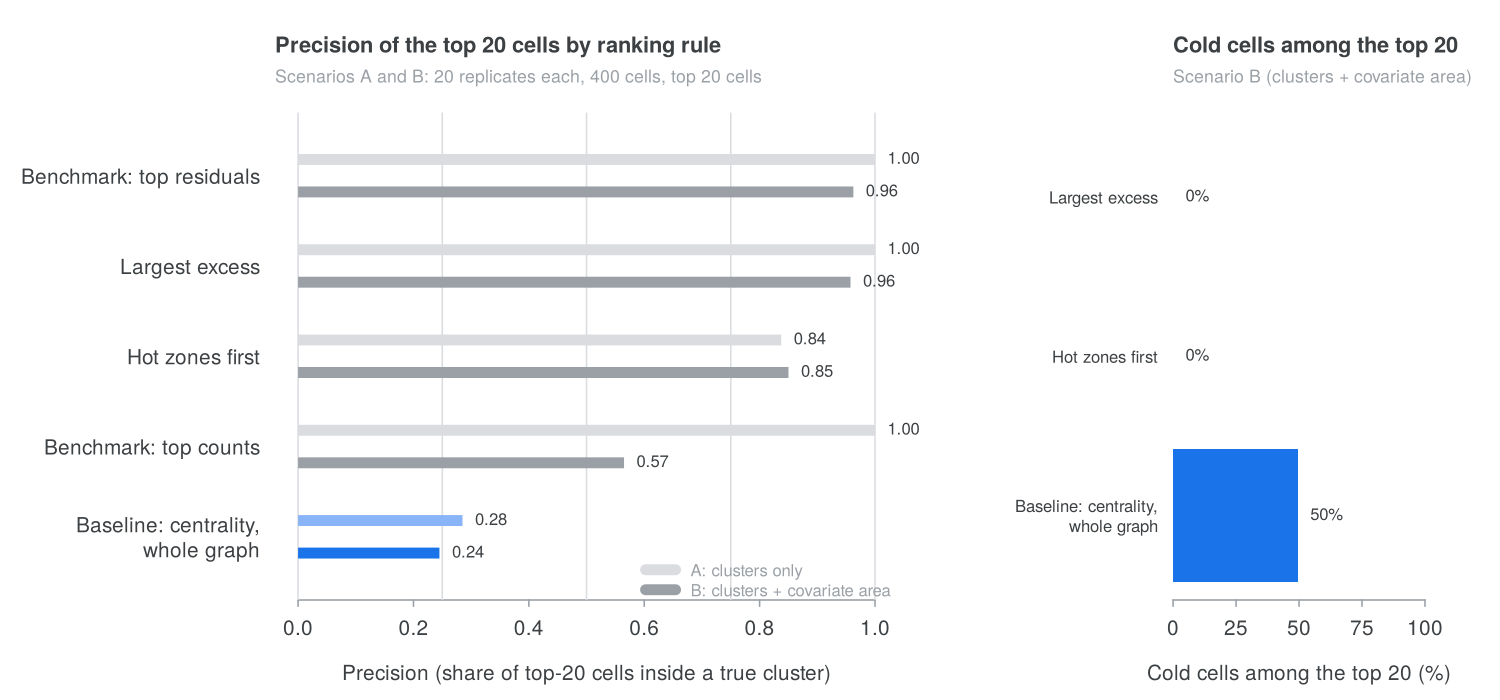
\includegraphics[width=\textwidth]{fig1_cold_zones}
\caption{Precision of the top 20 of 400 cells by ranking rule (scenarios A and B, 20 replicates each) and share of cold cells among them (scenario B). Baseline: harmonic centrality on the final graph.}
\label{fig:app-cold}
\end{figure}

\begin{figure}[ht]
\centering
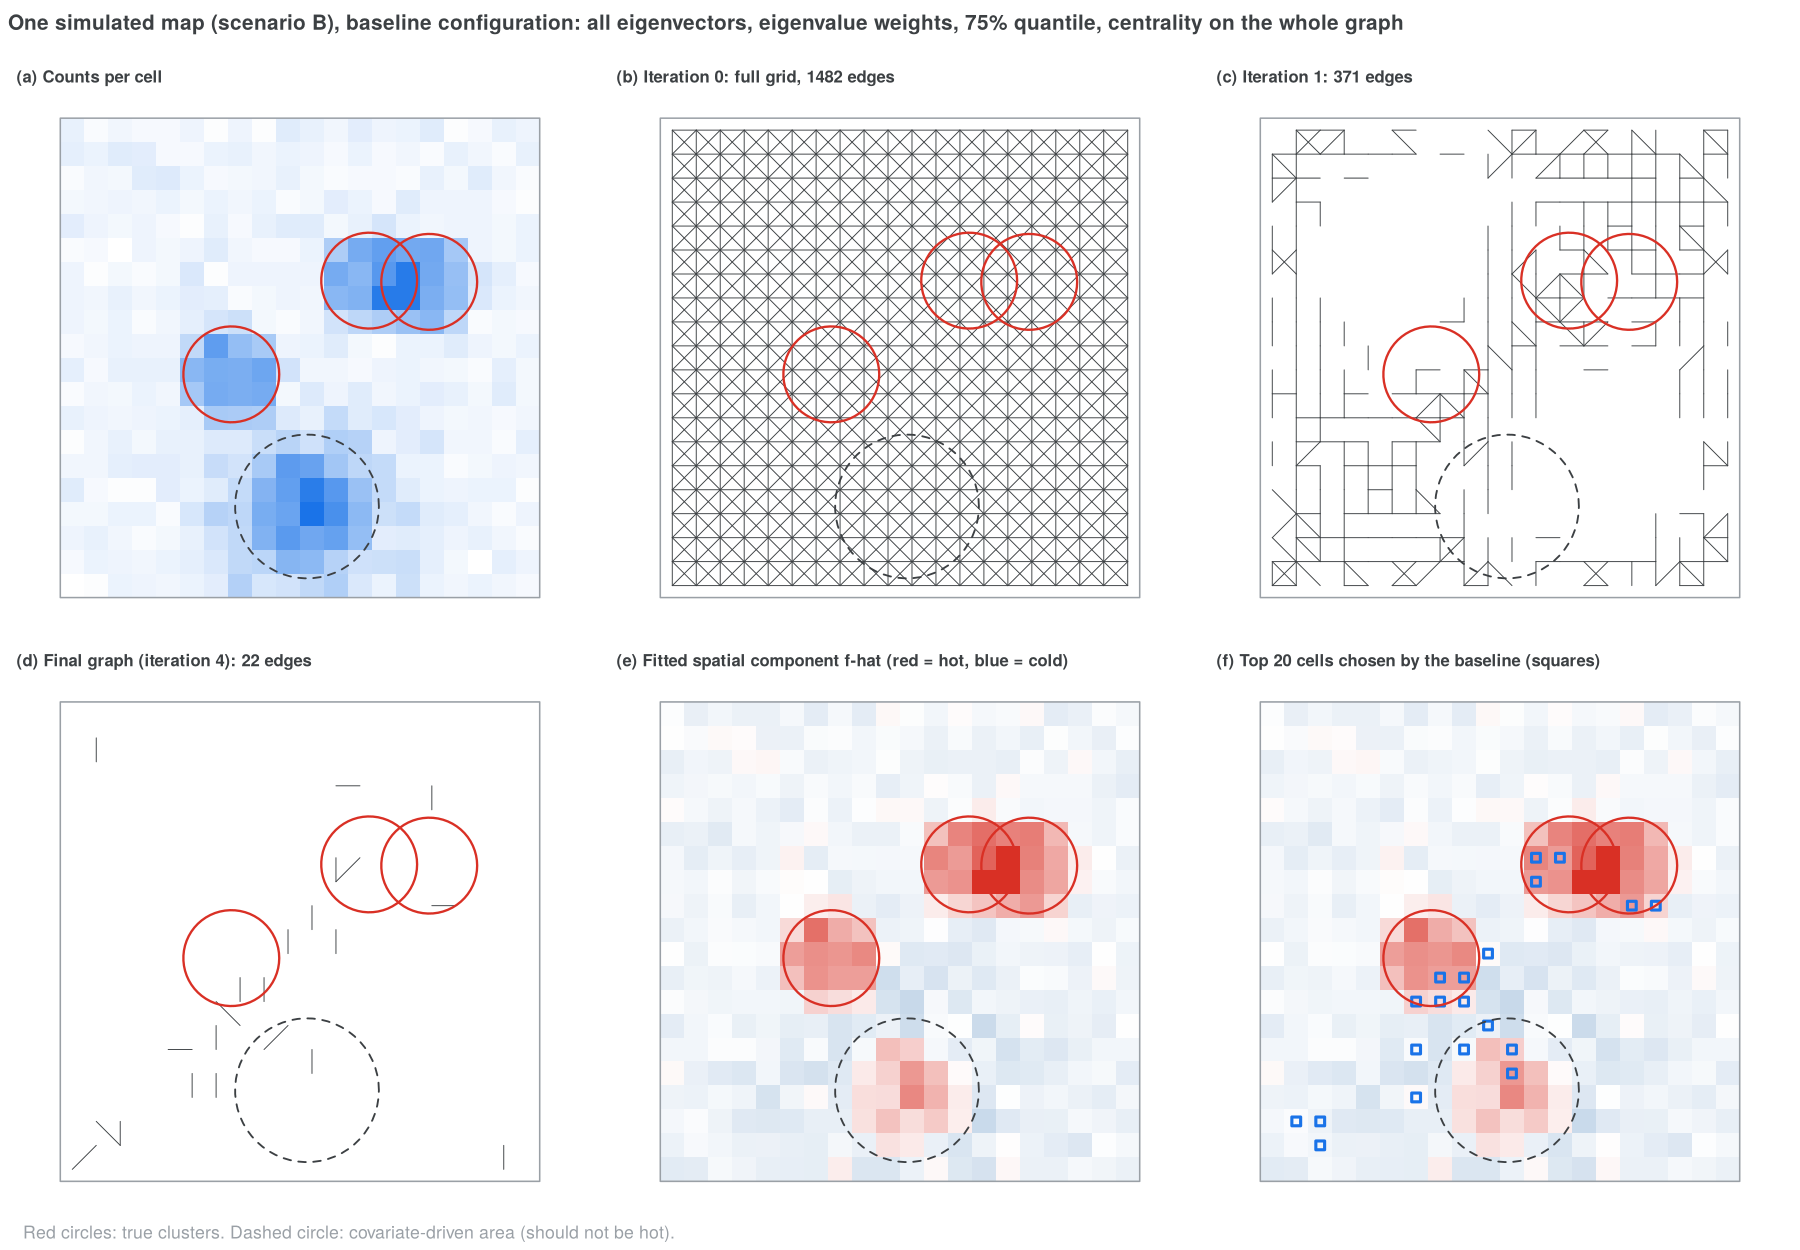
\includegraphics[width=\textwidth]{figS2_example_run}
\caption{One simulated map from scenario B under the baseline configuration. (a) Counts per cell. (b)--(d) Graph at iterations 0, 1 and at the last accepted iteration. (e) Fitted spatial component $\hat f$. (f) Top 20 cells under the baseline ranking. Circles: true clusters; dashed circle: covariate area.}
\label{fig:app-example}
\end{figure}

\paragraph{Effect of rounding and iteration on the selected cells.}
We compared rounding with the 75\% quantile against no rounding over 162 settings of scenario B: grids of $10\times10$, $20\times20$ and $40\times40$ cells, 50, 200 or 500 points per cluster, penalty exponents $a\in\{0.5,1,2\}$ in $\lambda=|z_0|^{-a}$, counts on the original or the $\log(Y+1)$ scale, and three ranking rules (10 replicates per setting). Iteration removed edges in 495 of 1620 runs (31\%); in the remaining runs the first reduced graph was rejected by the Moran test. In the runs where edges were removed, the change in precision was $+0.06$ (95\% CI $0.02$ to $0.10$) for centrality on the whole graph, $-0.01$ ($-0.03$ to $0.01$) for largest excess and $-0.06$ ($-0.11$ to $-0.01$) for hot zones first (Fig.~\ref{fig:app-iteration}).

\begin{figure}[ht]
\centering
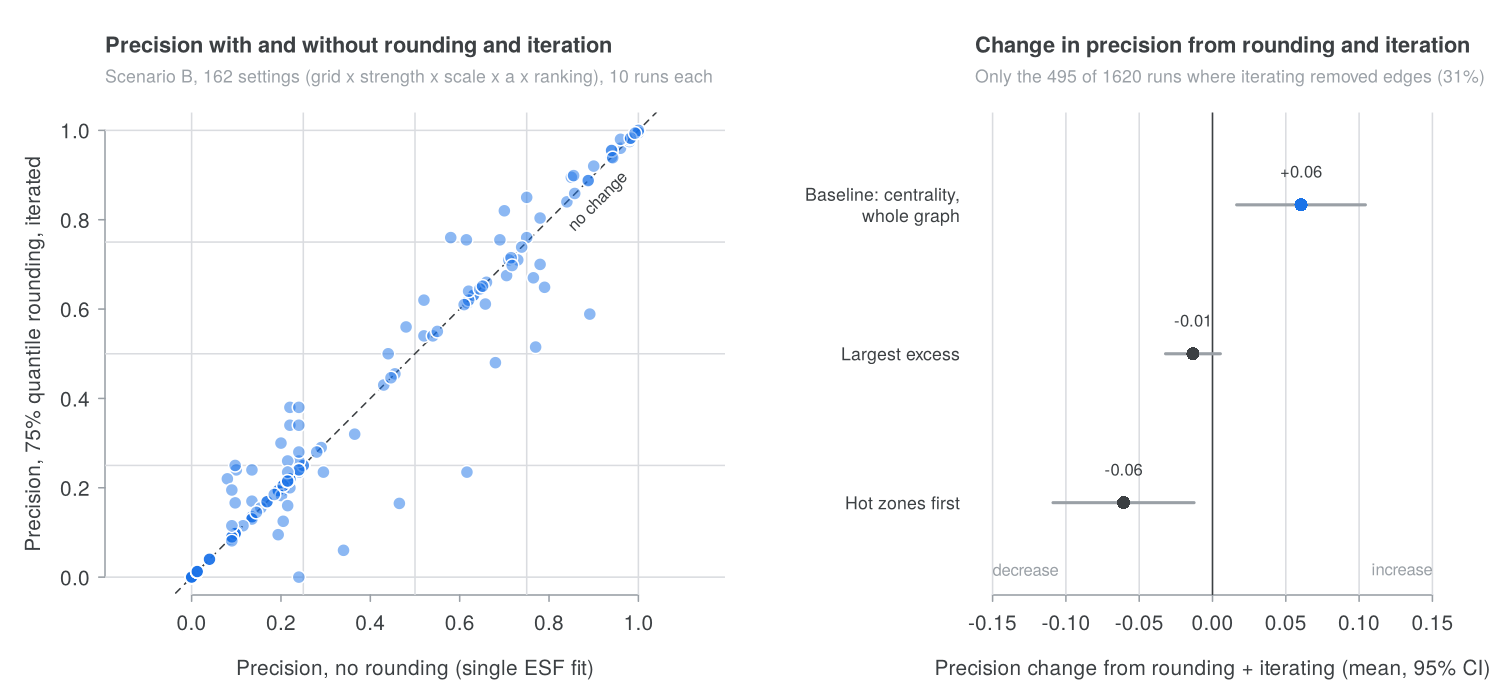
\includegraphics[width=\textwidth]{fig2_iteration_no_effect}
\caption{Left: precision with no rounding against precision with 75\% quantile rounding and iteration; each point is one setting (mean of 10 replicates). Right: change in precision in the runs where iteration removed edges (mean and 95\% confidence interval).}
\label{fig:app-iteration}
\end{figure}

\paragraph{Rounding rules.}
Table~\ref{tab:app-rounding} and Fig.~\ref{fig:app-rounding} compare the seven rounding rules with all other elements fixed at the baseline (scenarios A and B, 20 replicates each; scenarios D and D0, 20 replicates each). With the largest-excess ranking, precision was 1.00 in scenario A and 0.95--0.96 in scenario B for every rule, including no rounding. With hot zones first, the 80\% and 90\% quantiles and the permutation rule gave about 0.10 more than no rounding, and remained below the largest-excess ranking. With the baseline ranking, precision ranged from 0.10 to 0.37. In scenario D0 every rule except the mixture removed between 90\% and 97\% of the edges.

\begin{table}[ht]
\centering
\caption{Precision of the top 20 cells (scenario A / scenario B) by rounding rule and ranking rule, and share of edges kept in scenario D0. Mean of 20 replicates.}
\label{tab:app-rounding}
\small\setlength{\tabcolsep}{4pt}
\begin{tabular}{lcccc}
\hline
Rounding rule & Largest excess & Hot zones first & Centrality, & Edges kept \\
 & & & whole graph & (D0) \\
\hline
None            & 1.00 / 0.95 & 0.85 / 0.76 & 0.13 / 0.10 & 100\% \\
50\% quantile   & 1.00 / 0.95 & 0.81 / 0.71 & 0.32 / 0.37 & 6\% \\
75\% quantile (baseline) & 1.00 / 0.95 & 0.84 / 0.84 & 0.22 / 0.29 & 8\% \\
80\% quantile   & 1.00 / 0.95 & 0.89 / 0.90 & 0.19 / 0.31 & 3\% \\
90\% quantile   & 1.00 / 0.95 & 0.91 / 0.91 & 0.26 / 0.32 & 10\% \\
Mixture         & 1.00 / 0.96 & 0.80 / 0.78 & 0.26 / 0.31 & 76\% \\
Permutation     & 1.00 / 0.95 & 0.90 / 0.91 & 0.23 / 0.37 & 10\% \\
\hline
\end{tabular}
\end{table}

\begin{figure}[ht]
\centering
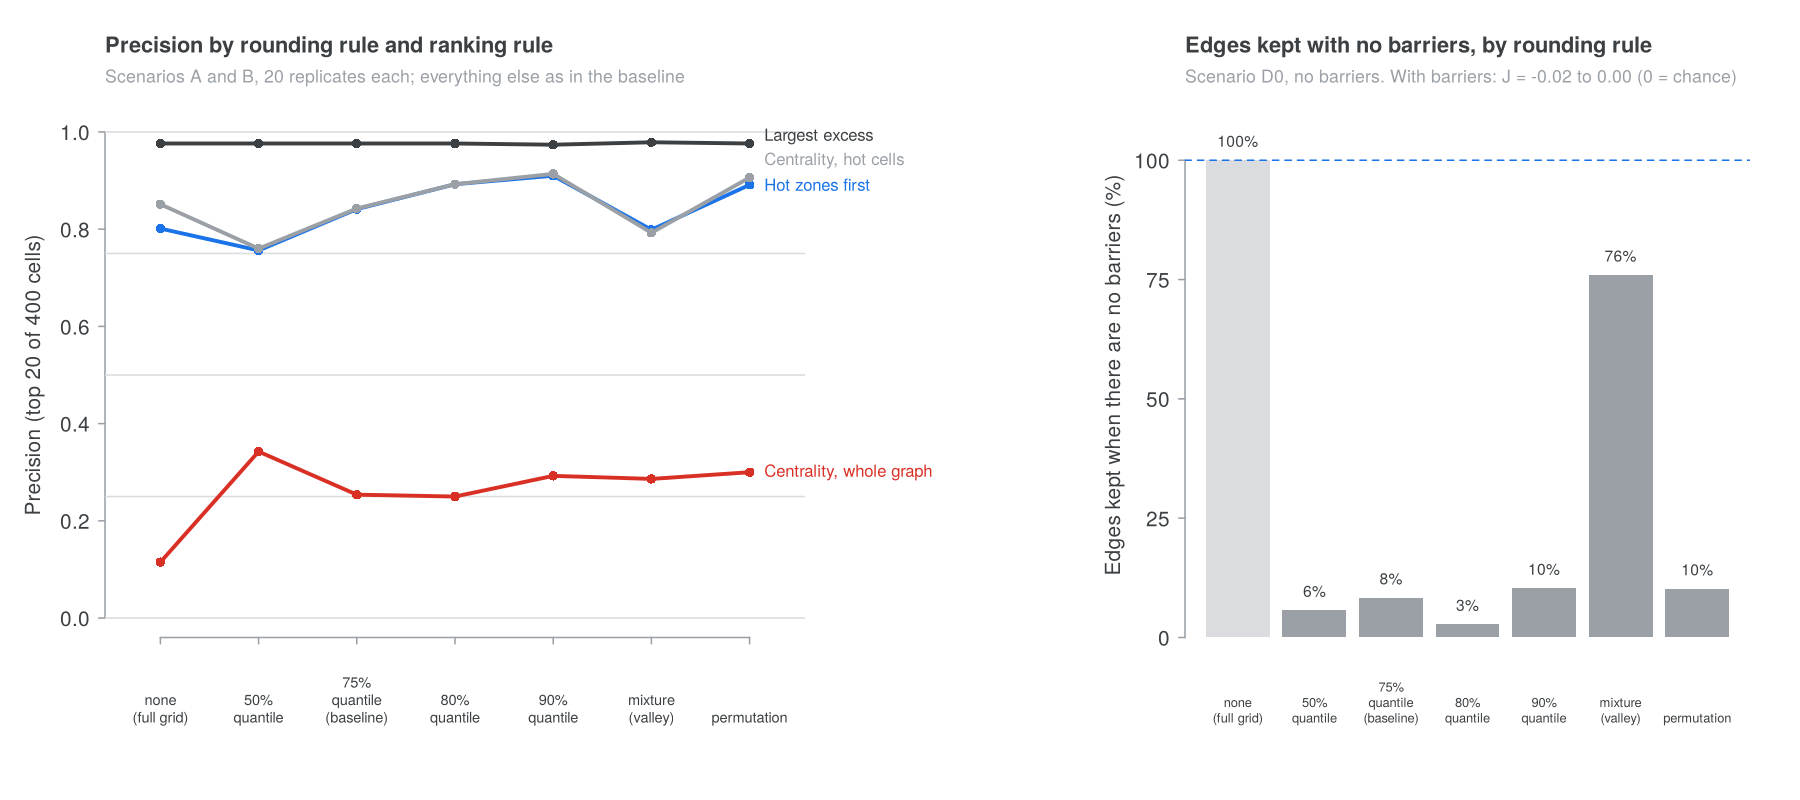
\includegraphics[width=\textwidth]{fig4_rounding_rules}
\caption{Left: precision of the top 20 of 400 cells by rounding rule and ranking rule (scenarios A and B pooled, 20 replicates each). Right: share of edges kept in scenario D0, where no edge should be removed.}
\label{fig:app-rounding}
\end{figure}

\paragraph{Fine grid with weak clusters.}
On a $40\times40$ grid (cell side 25) with 50 or 200 points per cluster, scenario B, budget of 80 cells, 10 replicates, the rankings that use hot cells and connectivity reached, with no rounding, a precision of 0.44--0.48 (50 points) and 0.81--0.89 (200 points), against 0.29 and 0.80 for top residuals on the log scale. Rounding reduced the precision of hot zones first by 0.24 and 0.25 (75\% quantile), 0.18 and 0.17 (90\% quantile) and 0.06 and 0.10 (permutation) (Fig.~\ref{fig:app-finegrid}).

\begin{figure}[ht]
\centering
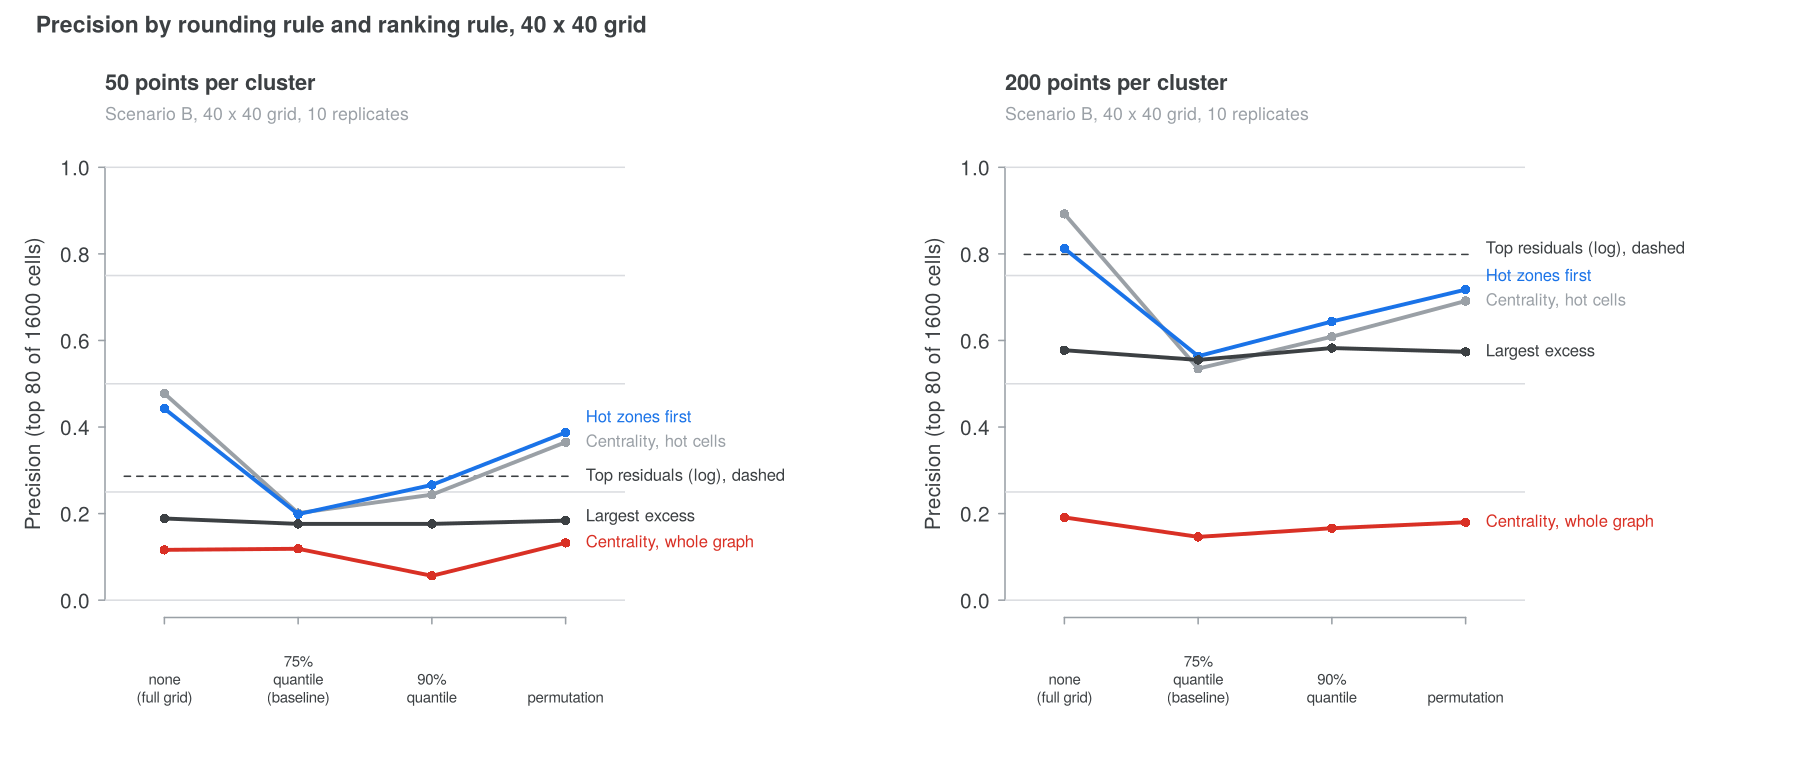
\includegraphics[width=\textwidth]{fig5_fine_grid}
\caption{Precision of the top 80 of 1600 cells by rounding rule and ranking rule on a $40\times40$ grid (scenario B, 10 replicates per panel). Dashed line: top residuals of $\log(Y+1)$ on $Z$.}
\label{fig:app-finegrid}
\end{figure}

\paragraph{Recovery of a known graph.}
In scenario D, the AUC of $b_{ij}$ for separating real from barrier edges was 0.55, 0.55 and 0.45 for $\rho=0.5$, $0.8$ and $0.95$ with eigenvalue weights, and 0.55, 0.53 and 0.61 with squared coefficients $\hat\gamma_s^2$ as weights. The absolute difference between the residuals of neighbouring cells, $|e_i-e_j|$, gave 0.55, 0.65 and 0.96 (Fig.~\ref{fig:app-graph}). After the full procedure, Youden's $J$ ranged from $-0.02$ to $0.00$ across rounding rules. With 130--300 of 400 eigenvectors selected, $B$ differs from $A$ by a small number of patterns with global support, while a barrier is a local discontinuity.

\begin{figure}[ht]
\centering
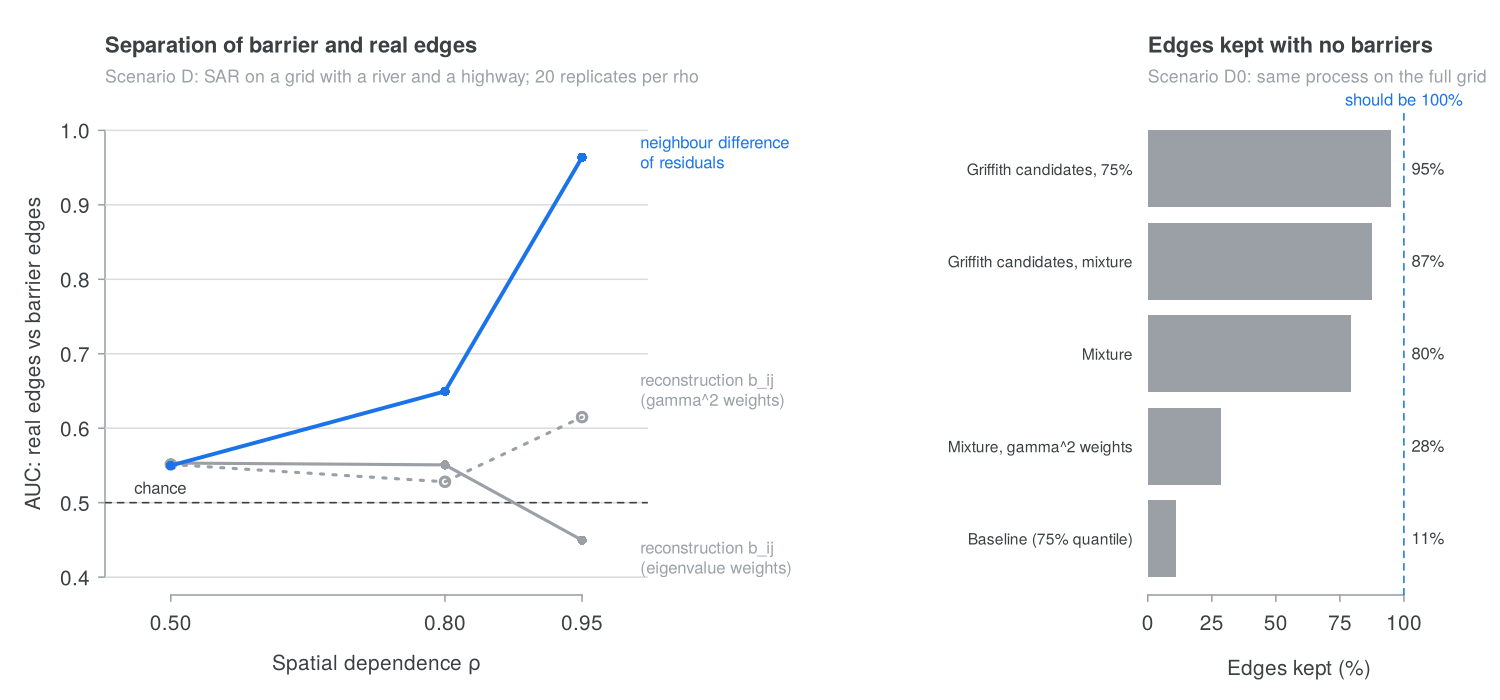
\includegraphics[width=\textwidth]{fig3_latent_graph}
\caption{Left: AUC for separating real edges from barrier edges in scenario D (20 replicates per $\rho$). Right: share of edges kept in scenario D0 by variant of the procedure.}
\label{fig:app-graph}
\end{figure}

\subsection{Conclusion}
\label{app:rec-conclusion}

In these simulations, no rounding rule increased the highest precision obtained without rounding by more than 0.01 (largest excess on the $20\times20$ grid; centrality among hot cells on the $40\times40$ grid). The reconstructed weights did not identify the edges removed by barriers, and most rounding rules removed most edges when no barrier was present. Ranking by centrality on the whole reconstructed graph selected cold cells in about half of the positions. The proposed procedure therefore uses the ESF step once, to estimate the spatial component $\hat f$ conditional on the covariates, and derives hot and cold zones from it on the contiguity graph $A$.

% Figures are read from ../simulation/figures/ (set in the preamble with
%     \graphicspath{{../simulation/figures/}}
% or copy the PNG files next to the .tex file).
% Packages used: graphicx, amsmath (both loaded by sn-jnl).
% Figures and tables are produced by simulation/04_iteration_figures.R from the
% results of simulation/01_ ... 06_*.R in the project repository.
% =====================================================================

\section{Iterative reconstruction of the spatial weights matrix}
\label{app:reconstruction}

This appendix describes an extension of the eigenvector spatial filtering (ESF) step that reconstructs a sparser spatial weights matrix from the selected eigenvectors and iterates the selection on the reconstructed graph. We evaluate it in simulation and explain why it is not part of the proposed procedure.

\subsection{The iterative reconstruction}
\label{app:rec-procedure}

Let $A$ be the $n\times n$ binary contiguity matrix of the study region, $Y$ the standardised counts per cell and $Z$ the standardised covariates. The procedure starts from $D^{(0)}=A$ and, at iteration $k$:

\begin{enumerate}
  \item computes the eigendecomposition $D^{(k)} = E\,\Delta\,E^\top$, with $\Delta=\mathrm{diag}(\delta_1,\dots,\delta_n)$, and selects a subset $S$ of eigenvectors with the MI-Lasso estimator, with penalty $\lambda=|z_0|^{-2}$ fixed from the standardised Moran's $I$ of the residuals of $Y$ on $Z$;
  \item reconstructs
  \begin{equation}
    B = E_S\,\Delta_S\,E_S^\top, \qquad b_{ij} = \sum_{s\in S}\delta_s\, e_s(i)\, e_s(j);
    \label{eq:app-B}
  \end{equation}
  \item applies a rounding rule: among the edges of $D^{(k)}$ with $b_{ij}>0$, it keeps those with $b_{ij}\ge\tau^{(k)}$, where $\tau^{(k)}$ is a threshold computed from these values, giving $D^{(k+1)} = D^{(k)}\circ\mathbf{1}\{B\ge\tau^{(k)}\}$;
  \item accepts $D^{(k+1)}$ if the post-Lasso residuals obtained with its eigenvectors show no spatial correlation (Moran's $I$ with $A$, level $0.05$), and stops otherwise or when $D^{(k+1)}=D^{(k)}$.
\end{enumerate}

Because each accepted step removes at least one edge, the procedure stops after at most as many iterations as $A$ has edges. Cells are then ranked by a ranking rule applied to the final graph.

We call \emph{baseline configuration} the procedure with all $n$ eigenvectors as candidates, eigenvalue weights in \eqref{eq:app-B}, the 75\% quantile of the positive $b_{ij}$ as threshold, and cells ranked by harmonic centrality on the final graph. Each variant below changes one element of the baseline.

\paragraph{Rounding rules.}
\emph{None} (all edges kept, $D=A$; no reconstruction);
\emph{quantile $q$} ($\tau$ = $q$-quantile of the positive $b_{ij}$ on the current edges, $q\in\{0.50, 0.75, 0.80, 0.90\}$);
\emph{mixture} (a two-component Gaussian mixture fitted to the positive $b_{ij}$; $\tau$ is the point between the two means where the weighted component densities are equal, and all edges are kept when the Bayesian information criterion selects one component);
\emph{permutation} (30 Freedman--Lane permutations of the residuals of $Y$ on $Z$; for each, the selection and \eqref{eq:app-B} are recomputed on the current graph, and $\tau$ is the 95th percentile of the pooled positive $b_{ij}$).

\paragraph{Ranking rules.}
Let $\hat f = E_S\hat\gamma_S$ be the fitted spatial component (centred), and call a cell \emph{hot} if $\hat f_i>0$ and \emph{cold} otherwise.
\emph{Centrality, whole graph}: harmonic centrality on the final graph, over all cells (baseline).
\emph{Centrality, hot cells}: harmonic centrality computed among hot cells only.
\emph{Largest excess}: hot cells ordered by $\hat f_i$.
\emph{Hot zones first}: connected groups of hot cells ordered by $\sum_{i}\hat f_i$; within a group, cells ordered by harmonic centrality.
Two benchmarks that do not use the graph are also reported: \emph{top counts} (cells ordered by $Y$) and \emph{top residuals} (cells ordered by the residuals of $Y$, or of $\log(Y+1)$, on $Z$).

\subsection{Simulation design}
\label{app:rec-design}

All scenarios use a $1000\times1000$ window divided into a regular grid with queen contiguity. Table~\ref{tab:app-scenarios} lists the scenarios.

\begin{table}[ht]
\centering
\caption{Simulated scenarios.}
\label{tab:app-scenarios}
\begin{tabular}{p{0.16\textwidth}p{0.50\textwidth}p{0.24\textwidth}}
\hline
Scenario & Data-generating process & Target \\
\hline
A: clusters & Three clusters: parents uniform in the window at least 100 units from the border; 500 offspring per parent, uniform in a disc of radius 100; 2000 additional uniform points. No covariate. & Cells inside the three discs \\
B: clusters and covariate & Scenario A plus 3000 points accepted with probability $\exp\{3(b(x)-1)\}$, where $b$ is a Gaussian surface (standard deviation 150) centred at least 300 units from every parent. The model receives $Z=(b,\ \varepsilon)$ at the cell centres, with $\varepsilon\sim N(0,1)$. & Cells inside the three discs, not the covariate area \\
D: barriers & $Y=\rho W Y + Z\beta + e$ on a $20\times20$ grid, with $W$ the row-standardised version of a graph $W^\ast\subset A$ in which a vertical line (one crossing left open) and a horizontal line on the left half remove 85 of the 1482 edges; $Z$ a linear gradient and noise, $\beta=(1,0)$, $\rho\in\{0.5,0.8,0.95\}$. & The 85 removed edges \\
D0: no barriers & As D with $W^\ast=A$. & No edge removed \\
\hline
\end{tabular}
\end{table}

Unless stated otherwise the grid has $20\times20$ cells (cell side 50) and the budget is the top 20 cells (5\%). For scenarios A and B, \emph{precision} is the share of the selected cells inside a true cluster disc. For scenarios D and D0, edges are classified as kept or removed, and we report the area under the ROC curve (AUC) of $b_{ij}$ for separating real from barrier edges, the share of edges kept, and Youden's $J$ = (share of barrier edges removed) + (share of real edges kept) $-\,1$, which is 0 for a classification unrelated to the barriers.

\subsection{Results}
\label{app:rec-results}

\paragraph{Sign of the reconstructed weights.}
Equation~\eqref{eq:app-B} is invariant to the sign of each eigenvector, since $e_s e_s^\top=(-e_s)(-e_s)^\top$. A positive $b_{ij}$ indicates that cells $i$ and $j$ lie on the same side of the selected spatial patterns, whether both have high or both have low counts. Under the baseline configuration, half of the 20 cells ranked highest in scenario B had $\hat f_i<0$, and precision was 0.28 in scenario A and 0.24 in scenario B (Fig.~\ref{fig:app-cold}). Ranking hot cells by $\hat f$ gave 1.00 and 0.96. Figure~\ref{fig:app-example} shows the successive graphs and the selected cells for one simulated map.

\begin{figure}[ht]
\centering
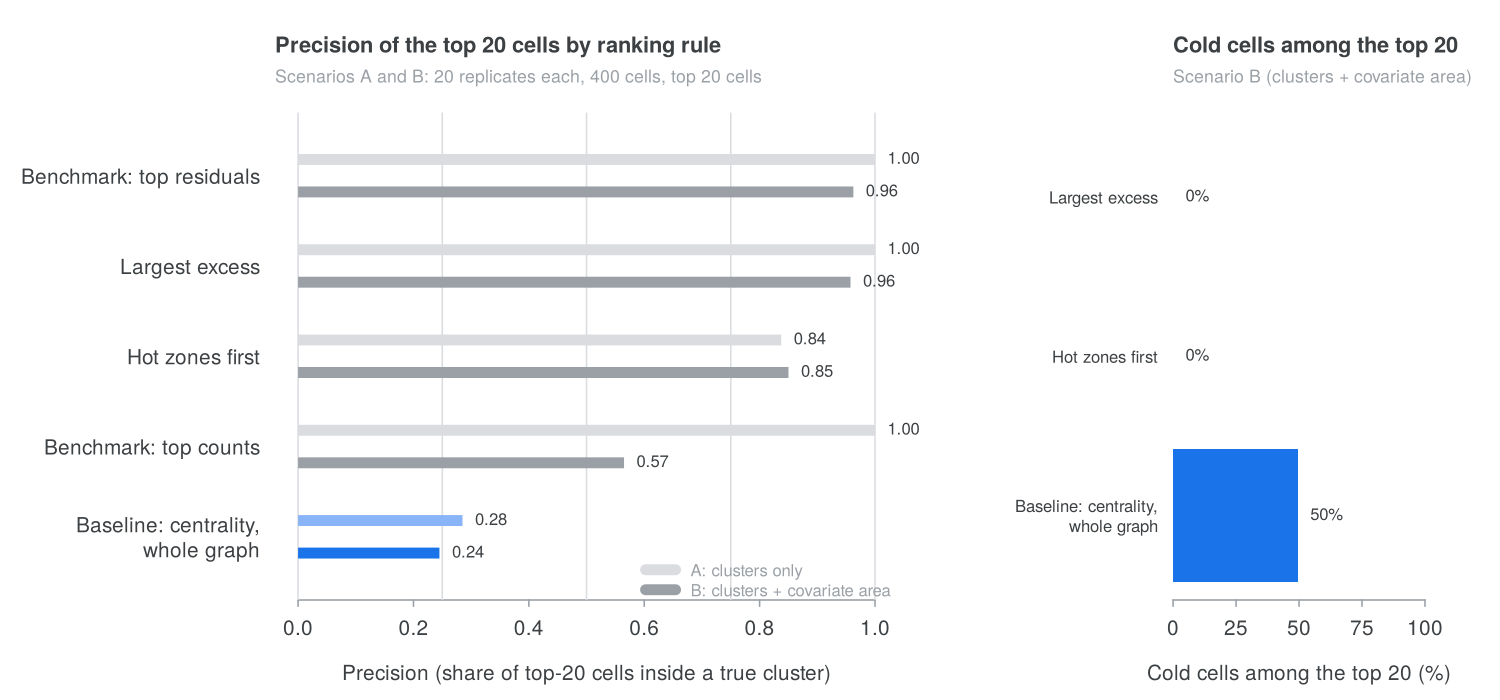
\includegraphics[width=\textwidth]{fig1_cold_zones}
\caption{Precision of the top 20 of 400 cells by ranking rule (scenarios A and B, 20 replicates each) and share of cold cells among them (scenario B). Baseline: harmonic centrality on the final graph.}
\label{fig:app-cold}
\end{figure}

\begin{figure}[ht]
\centering
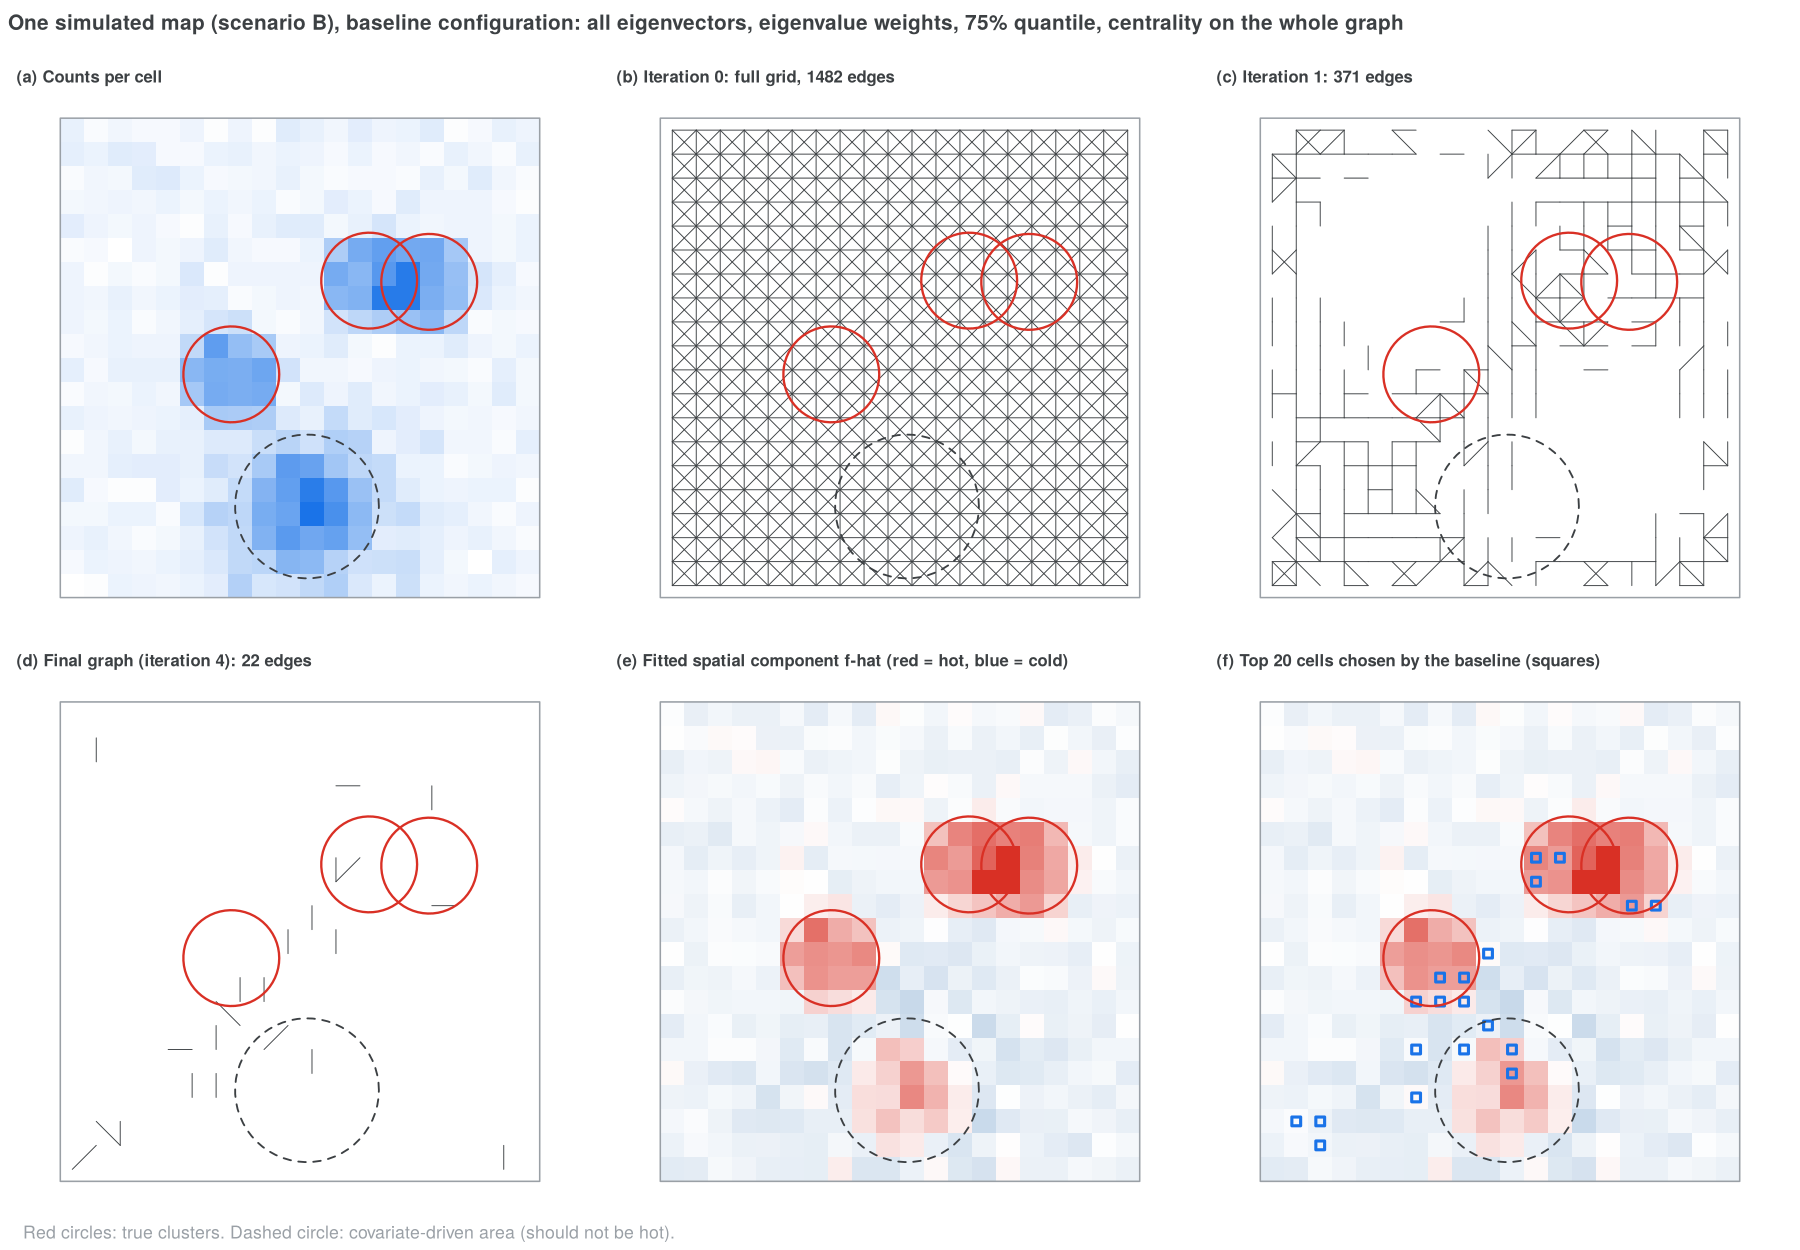
\includegraphics[width=\textwidth]{figS2_example_run}
\caption{One simulated map from scenario B under the baseline configuration. (a) Counts per cell. (b)--(d) Graph at iterations 0, 1 and at the last accepted iteration. (e) Fitted spatial component $\hat f$. (f) Top 20 cells under the baseline ranking. Circles: true clusters; dashed circle: covariate area.}
\label{fig:app-example}
\end{figure}

\paragraph{Effect of rounding and iteration on the selected cells.}
We compared rounding with the 75\% quantile against no rounding over 162 settings of scenario B: grids of $10\times10$, $20\times20$ and $40\times40$ cells, 50, 200 or 500 points per cluster, penalty exponents $a\in\{0.5,1,2\}$ in $\lambda=|z_0|^{-a}$, counts on the original or the $\log(Y+1)$ scale, and three ranking rules (10 replicates per setting). Iteration removed edges in 495 of 1620 runs (31\%); in the remaining runs the first reduced graph was rejected by the Moran test. In the runs where edges were removed, the change in precision was $+0.06$ (95\% CI $0.02$ to $0.10$) for centrality on the whole graph, $-0.01$ ($-0.03$ to $0.01$) for largest excess and $-0.06$ ($-0.11$ to $-0.01$) for hot zones first (Fig.~\ref{fig:app-iteration}).

\begin{figure}[ht]
\centering
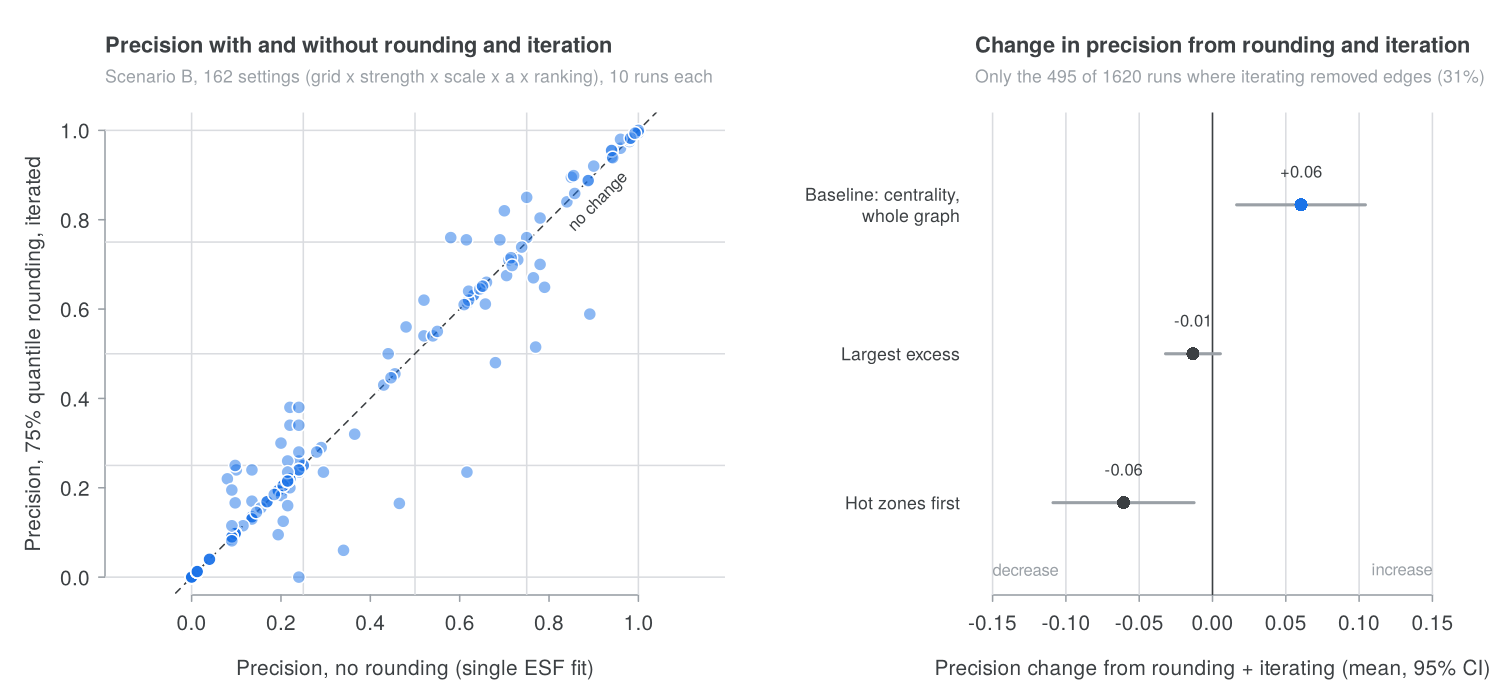
\includegraphics[width=\textwidth]{fig2_iteration_no_effect}
\caption{Left: precision with no rounding against precision with 75\% quantile rounding and iteration; each point is one setting (mean of 10 replicates). Right: change in precision in the runs where iteration removed edges (mean and 95\% confidence interval).}
\label{fig:app-iteration}
\end{figure}

\paragraph{Rounding rules.}
Table~\ref{tab:app-rounding} and Fig.~\ref{fig:app-rounding} compare the seven rounding rules with all other elements fixed at the baseline (scenarios A and B, 20 replicates each; scenarios D and D0, 20 replicates each). With the largest-excess ranking, precision was 1.00 in scenario A and 0.95--0.96 in scenario B for every rule, including no rounding. With hot zones first, the 80\% and 90\% quantiles and the permutation rule gave about 0.10 more than no rounding, and remained below the largest-excess ranking. With the baseline ranking, precision ranged from 0.10 to 0.37. In scenario D0 every rule except the mixture removed between 90\% and 97\% of the edges.

\begin{table}[ht]
\centering
\caption{Precision of the top 20 cells (scenario A / scenario B) by rounding rule and ranking rule, and share of edges kept in scenario D0. Mean of 20 replicates.}
\label{tab:app-rounding}
\small\setlength{\tabcolsep}{4pt}
\begin{tabular}{lcccc}
\hline
Rounding rule & Largest excess & Hot zones first & Centrality, & Edges kept \\
 & & & whole graph & (D0) \\
\hline
None            & 1.00 / 0.95 & 0.85 / 0.76 & 0.13 / 0.10 & 100\% \\
50\% quantile   & 1.00 / 0.95 & 0.81 / 0.71 & 0.32 / 0.37 & 6\% \\
75\% quantile (baseline) & 1.00 / 0.95 & 0.84 / 0.84 & 0.22 / 0.29 & 8\% \\
80\% quantile   & 1.00 / 0.95 & 0.89 / 0.90 & 0.19 / 0.31 & 3\% \\
90\% quantile   & 1.00 / 0.95 & 0.91 / 0.91 & 0.26 / 0.32 & 10\% \\
Mixture         & 1.00 / 0.96 & 0.80 / 0.78 & 0.26 / 0.31 & 76\% \\
Permutation     & 1.00 / 0.95 & 0.90 / 0.91 & 0.23 / 0.37 & 10\% \\
\hline
\end{tabular}
\end{table}

\begin{figure}[ht]
\centering
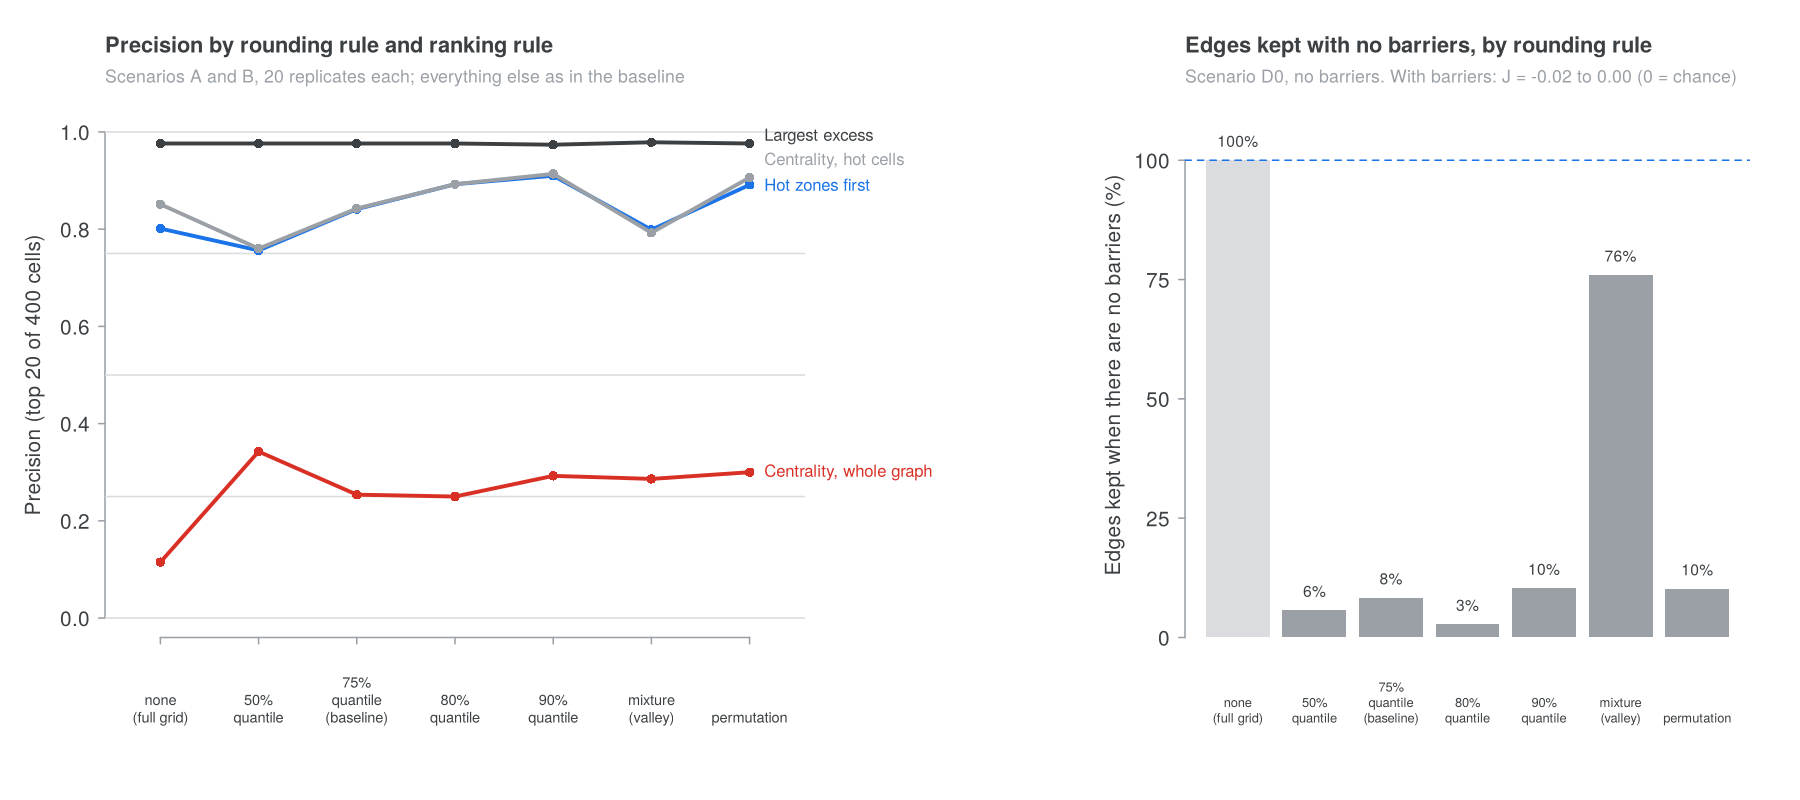
\includegraphics[width=\textwidth]{fig4_rounding_rules}
\caption{Left: precision of the top 20 of 400 cells by rounding rule and ranking rule (scenarios A and B pooled, 20 replicates each). Right: share of edges kept in scenario D0, where no edge should be removed.}
\label{fig:app-rounding}
\end{figure}

\paragraph{Fine grid with weak clusters.}
On a $40\times40$ grid (cell side 25) with 50 or 200 points per cluster, scenario B, budget of 80 cells, 10 replicates, the rankings that use hot cells and connectivity reached, with no rounding, a precision of 0.44--0.48 (50 points) and 0.81--0.89 (200 points), against 0.29 and 0.80 for top residuals on the log scale. Rounding reduced the precision of hot zones first by 0.24 and 0.25 (75\% quantile), 0.18 and 0.17 (90\% quantile) and 0.06 and 0.10 (permutation) (Fig.~\ref{fig:app-finegrid}).

\begin{figure}[ht]
\centering
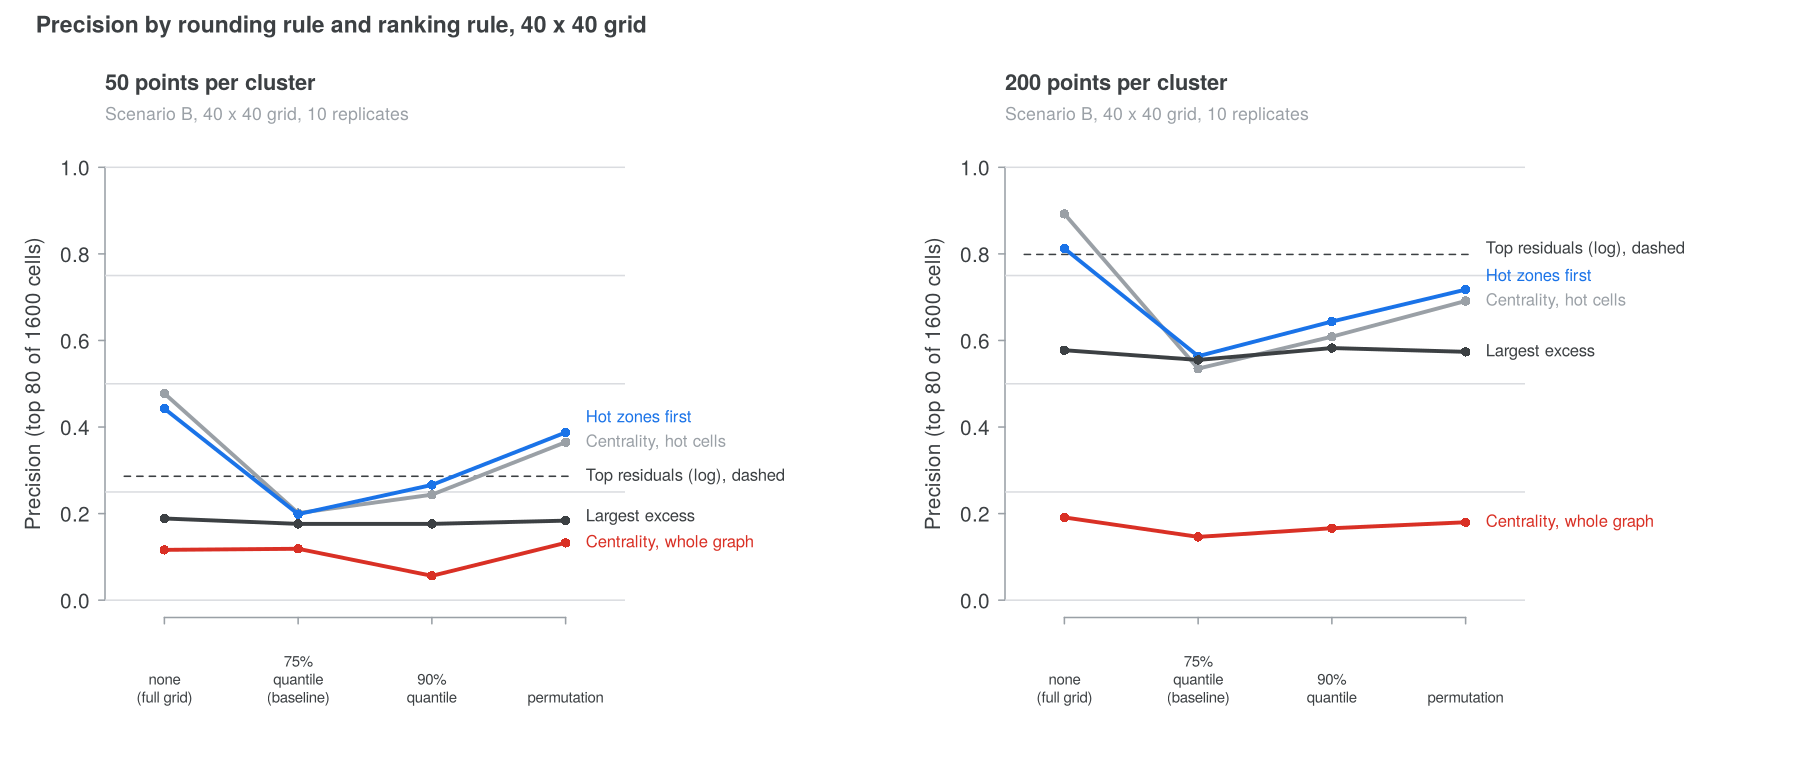
\includegraphics[width=\textwidth]{fig5_fine_grid}
\caption{Precision of the top 80 of 1600 cells by rounding rule and ranking rule on a $40\times40$ grid (scenario B, 10 replicates per panel). Dashed line: top residuals of $\log(Y+1)$ on $Z$.}
\label{fig:app-finegrid}
\end{figure}

\paragraph{Recovery of a known graph.}
In scenario D, the AUC of $b_{ij}$ for separating real from barrier edges was 0.55, 0.55 and 0.45 for $\rho=0.5$, $0.8$ and $0.95$ with eigenvalue weights, and 0.55, 0.53 and 0.61 with squared coefficients $\hat\gamma_s^2$ as weights. The absolute difference between the residuals of neighbouring cells, $|e_i-e_j|$, gave 0.55, 0.65 and 0.96 (Fig.~\ref{fig:app-graph}). After the full procedure, Youden's $J$ ranged from $-0.02$ to $0.00$ across rounding rules. With 130--300 of 400 eigenvectors selected, $B$ differs from $A$ by a small number of patterns with global support, while a barrier is a local discontinuity.

\begin{figure}[ht]
\centering
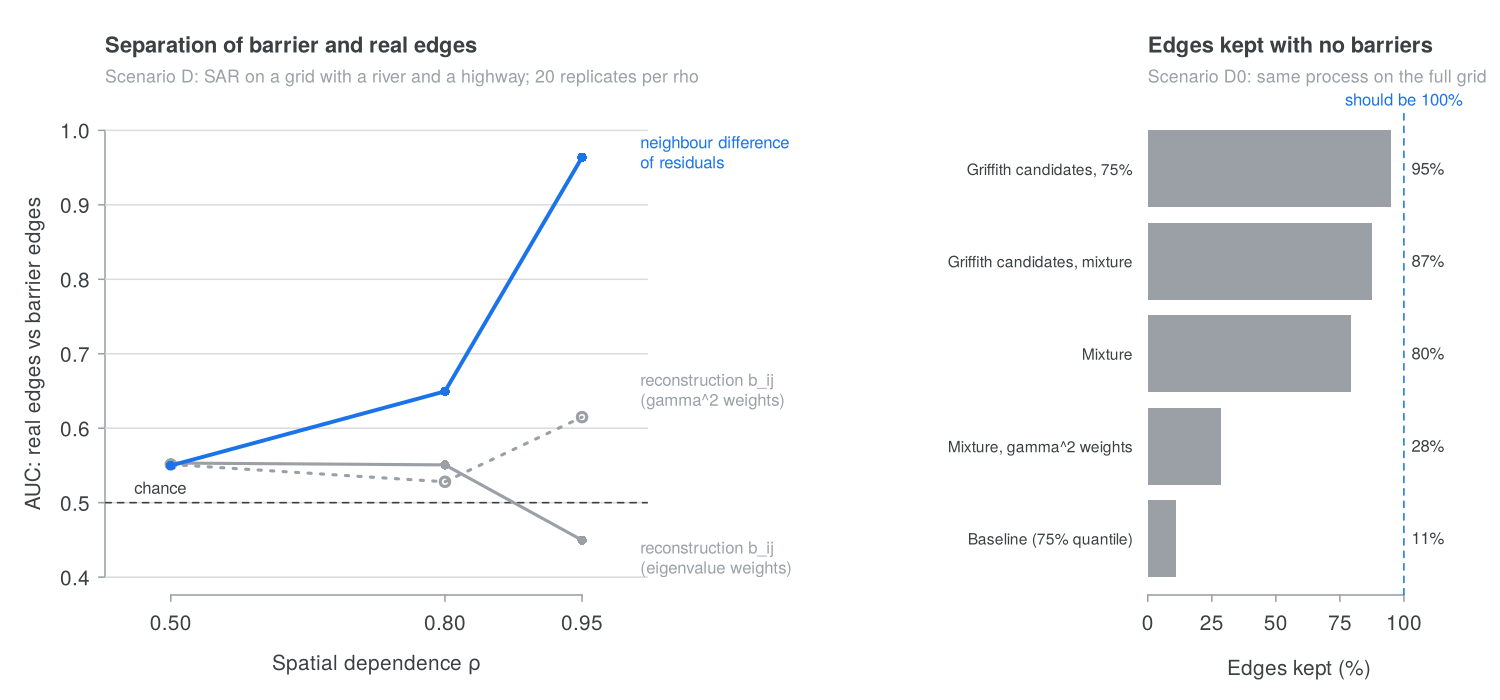
\includegraphics[width=\textwidth]{fig3_latent_graph}
\caption{Left: AUC for separating real edges from barrier edges in scenario D (20 replicates per $\rho$). Right: share of edges kept in scenario D0 by variant of the procedure.}
\label{fig:app-graph}
\end{figure}

\subsection{Conclusion}
\label{app:rec-conclusion}

In these simulations, no rounding rule increased the highest precision obtained without rounding by more than 0.01 (largest excess on the $20\times20$ grid; centrality among hot cells on the $40\times40$ grid). The reconstructed weights did not identify the edges removed by barriers, and most rounding rules removed most edges when no barrier was present. Ranking by centrality on the whole reconstructed graph selected cold cells in about half of the positions. The proposed procedure therefore uses the ESF step once, to estimate the spatial component $\hat f$ conditional on the covariates, and derives hot and cold zones from it on the contiguity graph $A$.

% Figures are read from ../simulation/figures/ (set in the preamble with
%     \graphicspath{{../simulation/figures/}}
% or copy the PNG files next to the .tex file).
% Packages used: graphicx, amsmath (both loaded by sn-jnl).
% Figures and tables are produced by simulation/04_iteration_figures.R from the
% results of simulation/01_ ... 06_*.R in the project repository.
% =====================================================================

\section{Iterative reconstruction of the spatial weights matrix}
\label{app:reconstruction}

This appendix describes an extension of the eigenvector spatial filtering (ESF) step that reconstructs a sparser spatial weights matrix from the selected eigenvectors and iterates the selection on the reconstructed graph. We evaluate it in simulation and explain why it is not part of the proposed procedure.

\subsection{The iterative reconstruction}
\label{app:rec-procedure}

Let $A$ be the $n\times n$ binary contiguity matrix of the study region, $Y$ the standardised counts per cell and $Z$ the standardised covariates. The procedure starts from $D^{(0)}=A$ and, at iteration $k$:

\begin{enumerate}
  \item computes the eigendecomposition $D^{(k)} = E\,\Delta\,E^\top$, with $\Delta=\mathrm{diag}(\delta_1,\dots,\delta_n)$, and selects a subset $S$ of eigenvectors with the MI-Lasso estimator, with penalty $\lambda=|z_0|^{-2}$ fixed from the standardised Moran's $I$ of the residuals of $Y$ on $Z$;
  \item reconstructs
  \begin{equation}
    B = E_S\,\Delta_S\,E_S^\top, \qquad b_{ij} = \sum_{s\in S}\delta_s\, e_s(i)\, e_s(j);
    \label{eq:app-B}
  \end{equation}
  \item applies a rounding rule: among the edges of $D^{(k)}$ with $b_{ij}>0$, it keeps those with $b_{ij}\ge\tau^{(k)}$, where $\tau^{(k)}$ is a threshold computed from these values, giving $D^{(k+1)} = D^{(k)}\circ\mathbf{1}\{B\ge\tau^{(k)}\}$;
  \item accepts $D^{(k+1)}$ if the post-Lasso residuals obtained with its eigenvectors show no spatial correlation (Moran's $I$ with $A$, level $0.05$), and stops otherwise or when $D^{(k+1)}=D^{(k)}$.
\end{enumerate}

Because each accepted step removes at least one edge, the procedure stops after at most as many iterations as $A$ has edges. Cells are then ranked by a ranking rule applied to the final graph.

We call \emph{baseline configuration} the procedure with all $n$ eigenvectors as candidates, eigenvalue weights in \eqref{eq:app-B}, the 75\% quantile of the positive $b_{ij}$ as threshold, and cells ranked by harmonic centrality on the final graph. Each variant below changes one element of the baseline.

\paragraph{Rounding rules.}
\emph{None} (all edges kept, $D=A$; no reconstruction);
\emph{quantile $q$} ($\tau$ = $q$-quantile of the positive $b_{ij}$ on the current edges, $q\in\{0.50, 0.75, 0.80, 0.90\}$);
\emph{mixture} (a two-component Gaussian mixture fitted to the positive $b_{ij}$; $\tau$ is the point between the two means where the weighted component densities are equal, and all edges are kept when the Bayesian information criterion selects one component);
\emph{permutation} (30 Freedman--Lane permutations of the residuals of $Y$ on $Z$; for each, the selection and \eqref{eq:app-B} are recomputed on the current graph, and $\tau$ is the 95th percentile of the pooled positive $b_{ij}$).

\paragraph{Ranking rules.}
Let $\hat f = E_S\hat\gamma_S$ be the fitted spatial component (centred), and call a cell \emph{hot} if $\hat f_i>0$ and \emph{cold} otherwise.
\emph{Centrality, whole graph}: harmonic centrality on the final graph, over all cells (baseline).
\emph{Centrality, hot cells}: harmonic centrality computed among hot cells only.
\emph{Largest excess}: hot cells ordered by $\hat f_i$.
\emph{Hot zones first}: connected groups of hot cells ordered by $\sum_{i}\hat f_i$; within a group, cells ordered by harmonic centrality.
Two benchmarks that do not use the graph are also reported: \emph{top counts} (cells ordered by $Y$) and \emph{top residuals} (cells ordered by the residuals of $Y$, or of $\log(Y+1)$, on $Z$).

\subsection{Simulation design}
\label{app:rec-design}

All scenarios use a $1000\times1000$ window divided into a regular grid with queen contiguity. Table~\ref{tab:app-scenarios} lists the scenarios.

\begin{table}[ht]
\centering
\caption{Simulated scenarios.}
\label{tab:app-scenarios}
\begin{tabular}{p{0.16\textwidth}p{0.50\textwidth}p{0.24\textwidth}}
\hline
Scenario & Data-generating process & Target \\
\hline
A: clusters & Three clusters: parents uniform in the window at least 100 units from the border; 500 offspring per parent, uniform in a disc of radius 100; 2000 additional uniform points. No covariate. & Cells inside the three discs \\
B: clusters and covariate & Scenario A plus 3000 points accepted with probability $\exp\{3(b(x)-1)\}$, where $b$ is a Gaussian surface (standard deviation 150) centred at least 300 units from every parent. The model receives $Z=(b,\ \varepsilon)$ at the cell centres, with $\varepsilon\sim N(0,1)$. & Cells inside the three discs, not the covariate area \\
D: barriers & $Y=\rho W Y + Z\beta + e$ on a $20\times20$ grid, with $W$ the row-standardised version of a graph $W^\ast\subset A$ in which a vertical line (one crossing left open) and a horizontal line on the left half remove 85 of the 1482 edges; $Z$ a linear gradient and noise, $\beta=(1,0)$, $\rho\in\{0.5,0.8,0.95\}$. & The 85 removed edges \\
D0: no barriers & As D with $W^\ast=A$. & No edge removed \\
\hline
\end{tabular}
\end{table}

Unless stated otherwise the grid has $20\times20$ cells (cell side 50) and the budget is the top 20 cells (5\%). For scenarios A and B, \emph{precision} is the share of the selected cells inside a true cluster disc. For scenarios D and D0, edges are classified as kept or removed, and we report the area under the ROC curve (AUC) of $b_{ij}$ for separating real from barrier edges, the share of edges kept, and Youden's $J$ = (share of barrier edges removed) + (share of real edges kept) $-\,1$, which is 0 for a classification unrelated to the barriers.

\subsection{Results}
\label{app:rec-results}

\paragraph{Sign of the reconstructed weights.}
Equation~\eqref{eq:app-B} is invariant to the sign of each eigenvector, since $e_s e_s^\top=(-e_s)(-e_s)^\top$. A positive $b_{ij}$ indicates that cells $i$ and $j$ lie on the same side of the selected spatial patterns, whether both have high or both have low counts. Under the baseline configuration, half of the 20 cells ranked highest in scenario B had $\hat f_i<0$, and precision was 0.28 in scenario A and 0.24 in scenario B (Fig.~\ref{fig:app-cold}). Ranking hot cells by $\hat f$ gave 1.00 and 0.96. Figure~\ref{fig:app-example} shows the successive graphs and the selected cells for one simulated map.

\begin{figure}[ht]
\centering
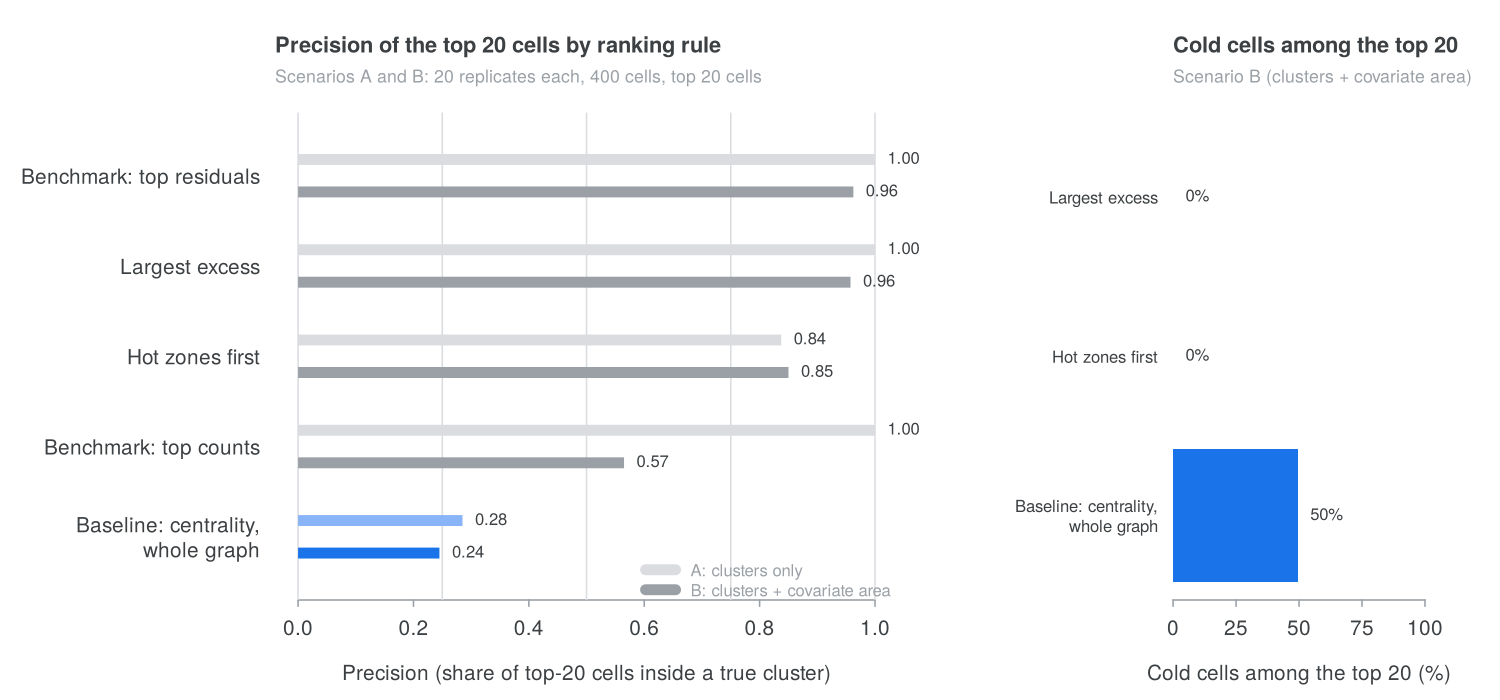
\includegraphics[width=\textwidth]{fig1_cold_zones}
\caption{Precision of the top 20 of 400 cells by ranking rule (scenarios A and B, 20 replicates each) and share of cold cells among them (scenario B). Baseline: harmonic centrality on the final graph.}
\label{fig:app-cold}
\end{figure}

\begin{figure}[ht]
\centering
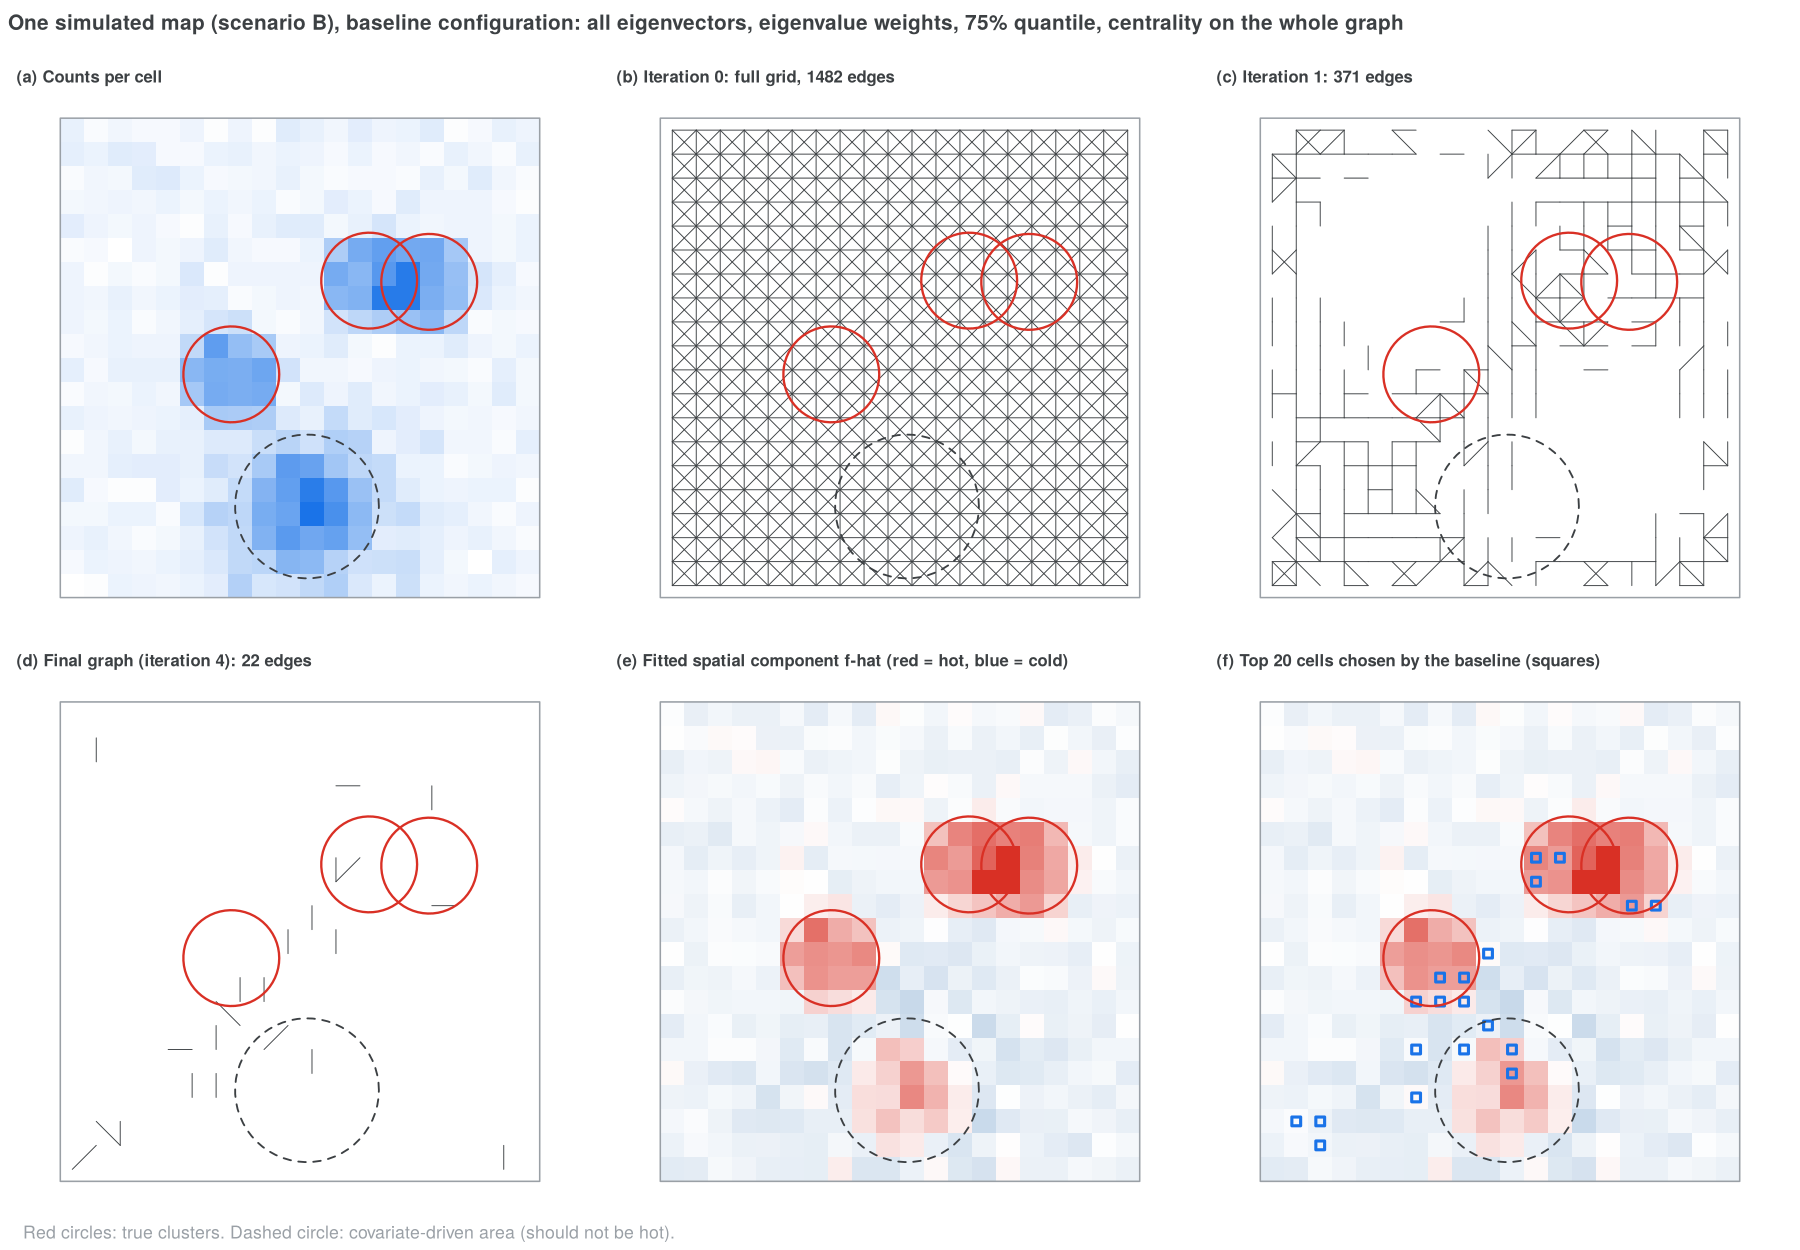
\includegraphics[width=\textwidth]{figS2_example_run}
\caption{One simulated map from scenario B under the baseline configuration. (a) Counts per cell. (b)--(d) Graph at iterations 0, 1 and at the last accepted iteration. (e) Fitted spatial component $\hat f$. (f) Top 20 cells under the baseline ranking. Circles: true clusters; dashed circle: covariate area.}
\label{fig:app-example}
\end{figure}

\paragraph{Effect of rounding and iteration on the selected cells.}
We compared rounding with the 75\% quantile against no rounding over 162 settings of scenario B: grids of $10\times10$, $20\times20$ and $40\times40$ cells, 50, 200 or 500 points per cluster, penalty exponents $a\in\{0.5,1,2\}$ in $\lambda=|z_0|^{-a}$, counts on the original or the $\log(Y+1)$ scale, and three ranking rules (10 replicates per setting). Iteration removed edges in 495 of 1620 runs (31\%); in the remaining runs the first reduced graph was rejected by the Moran test. In the runs where edges were removed, the change in precision was $+0.06$ (95\% CI $0.02$ to $0.10$) for centrality on the whole graph, $-0.01$ ($-0.03$ to $0.01$) for largest excess and $-0.06$ ($-0.11$ to $-0.01$) for hot zones first (Fig.~\ref{fig:app-iteration}).

\begin{figure}[ht]
\centering
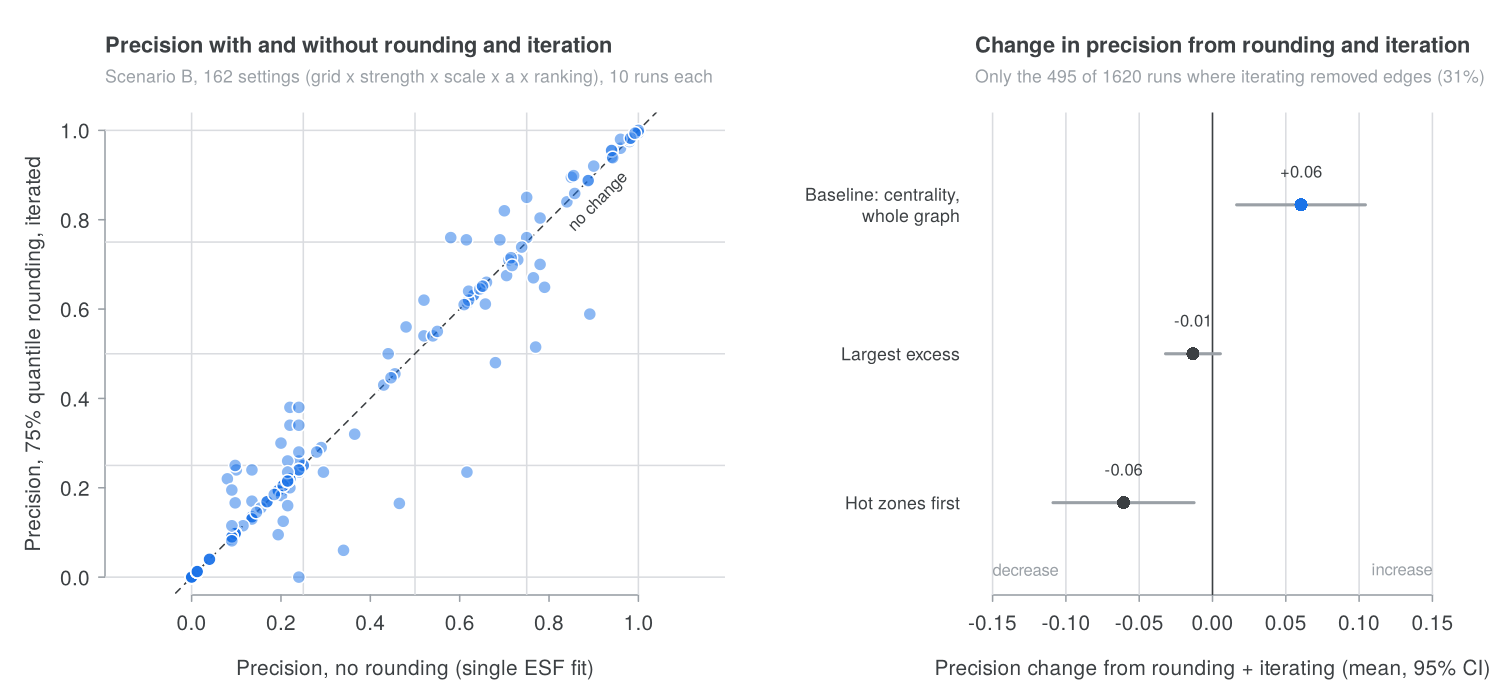
\includegraphics[width=\textwidth]{fig2_iteration_no_effect}
\caption{Left: precision with no rounding against precision with 75\% quantile rounding and iteration; each point is one setting (mean of 10 replicates). Right: change in precision in the runs where iteration removed edges (mean and 95\% confidence interval).}
\label{fig:app-iteration}
\end{figure}

\paragraph{Rounding rules.}
Table~\ref{tab:app-rounding} and Fig.~\ref{fig:app-rounding} compare the seven rounding rules with all other elements fixed at the baseline (scenarios A and B, 20 replicates each; scenarios D and D0, 20 replicates each). With the largest-excess ranking, precision was 1.00 in scenario A and 0.95--0.96 in scenario B for every rule, including no rounding. With hot zones first, the 80\% and 90\% quantiles and the permutation rule gave about 0.10 more than no rounding, and remained below the largest-excess ranking. With the baseline ranking, precision ranged from 0.10 to 0.37. In scenario D0 every rule except the mixture removed between 90\% and 97\% of the edges.

\begin{table}[ht]
\centering
\caption{Precision of the top 20 cells (scenario A / scenario B) by rounding rule and ranking rule, and share of edges kept in scenario D0. Mean of 20 replicates.}
\label{tab:app-rounding}
\small\setlength{\tabcolsep}{4pt}
\begin{tabular}{lcccc}
\hline
Rounding rule & Largest excess & Hot zones first & Centrality, & Edges kept \\
 & & & whole graph & (D0) \\
\hline
None            & 1.00 / 0.95 & 0.85 / 0.76 & 0.13 / 0.10 & 100\% \\
50\% quantile   & 1.00 / 0.95 & 0.81 / 0.71 & 0.32 / 0.37 & 6\% \\
75\% quantile (baseline) & 1.00 / 0.95 & 0.84 / 0.84 & 0.22 / 0.29 & 8\% \\
80\% quantile   & 1.00 / 0.95 & 0.89 / 0.90 & 0.19 / 0.31 & 3\% \\
90\% quantile   & 1.00 / 0.95 & 0.91 / 0.91 & 0.26 / 0.32 & 10\% \\
Mixture         & 1.00 / 0.96 & 0.80 / 0.78 & 0.26 / 0.31 & 76\% \\
Permutation     & 1.00 / 0.95 & 0.90 / 0.91 & 0.23 / 0.37 & 10\% \\
\hline
\end{tabular}
\end{table}

\begin{figure}[ht]
\centering
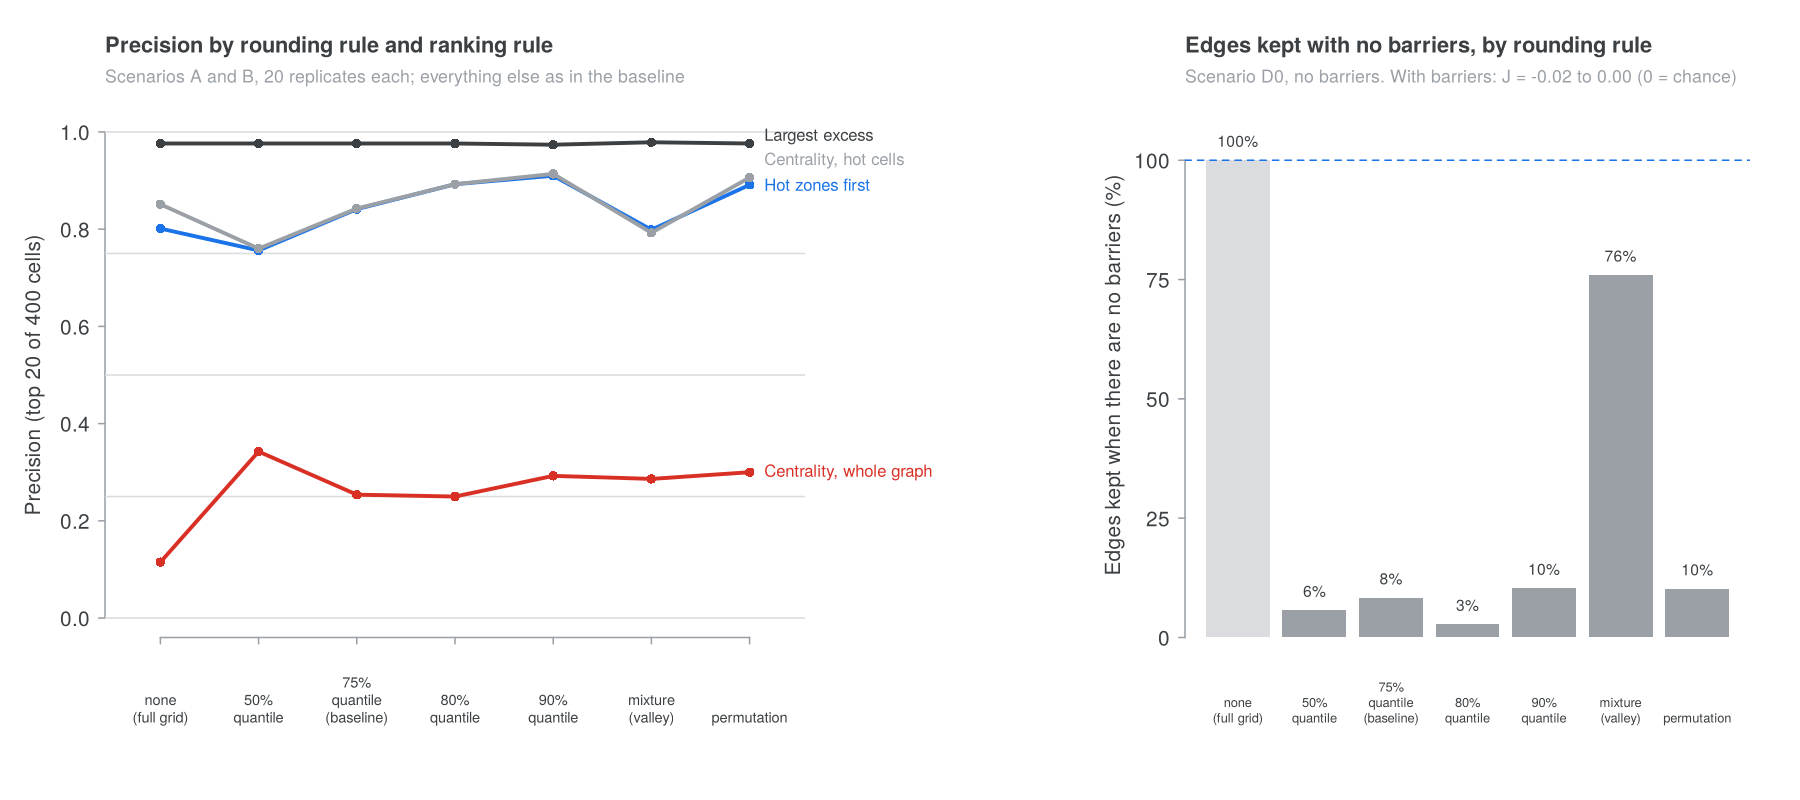
\includegraphics[width=\textwidth]{fig4_rounding_rules}
\caption{Left: precision of the top 20 of 400 cells by rounding rule and ranking rule (scenarios A and B pooled, 20 replicates each). Right: share of edges kept in scenario D0, where no edge should be removed.}
\label{fig:app-rounding}
\end{figure}

\paragraph{Fine grid with weak clusters.}
On a $40\times40$ grid (cell side 25) with 50 or 200 points per cluster, scenario B, budget of 80 cells, 10 replicates, the rankings that use hot cells and connectivity reached, with no rounding, a precision of 0.44--0.48 (50 points) and 0.81--0.89 (200 points), against 0.29 and 0.80 for top residuals on the log scale. Rounding reduced the precision of hot zones first by 0.24 and 0.25 (75\% quantile), 0.18 and 0.17 (90\% quantile) and 0.06 and 0.10 (permutation) (Fig.~\ref{fig:app-finegrid}).

\begin{figure}[ht]
\centering
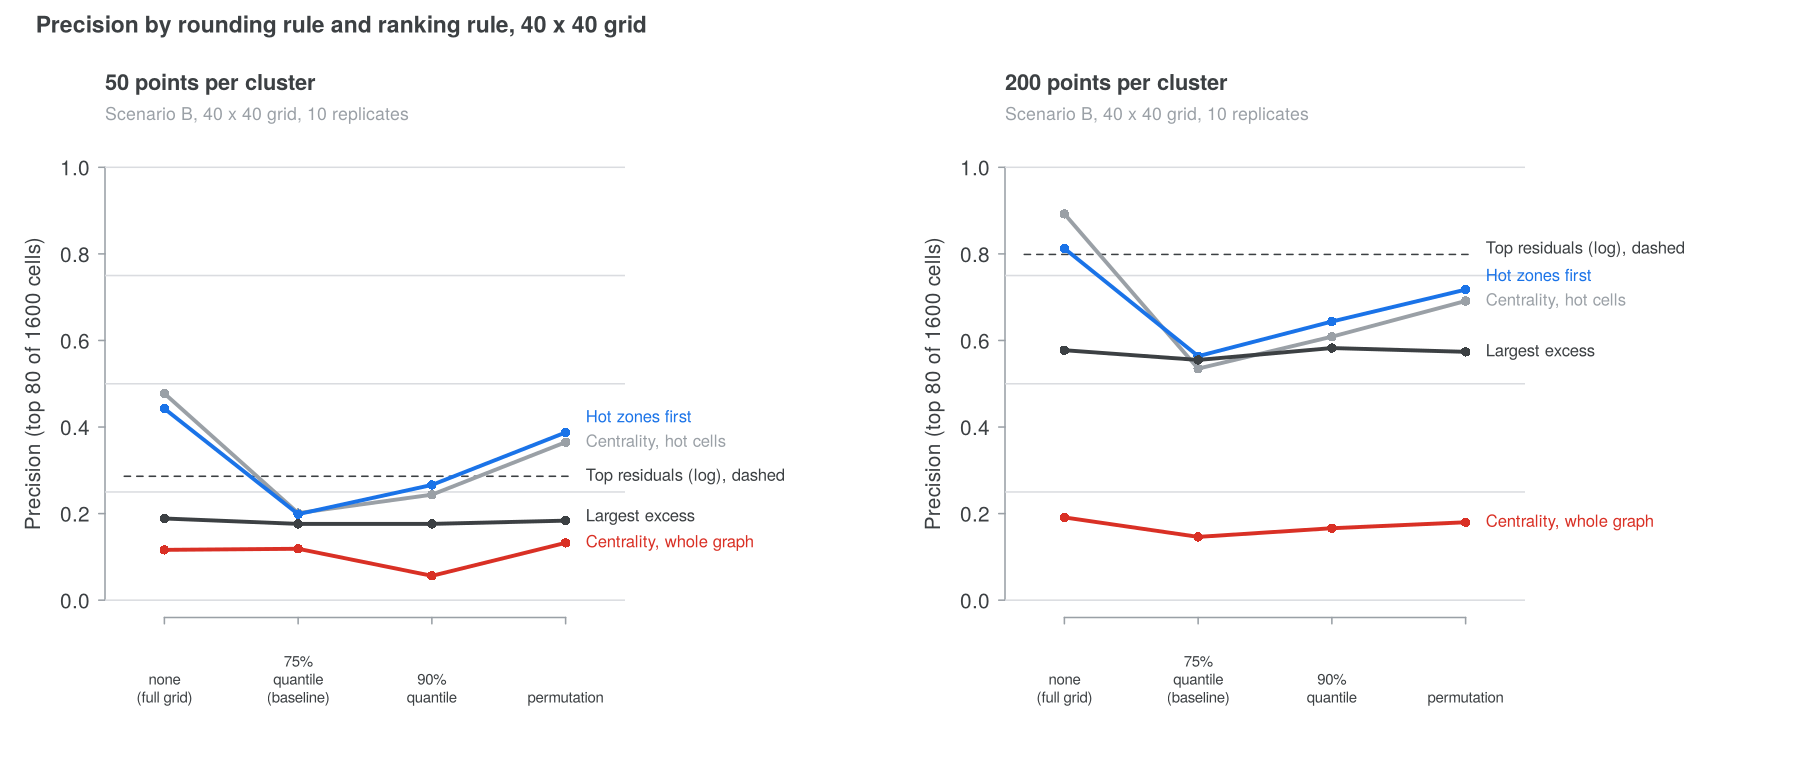
\includegraphics[width=\textwidth]{fig5_fine_grid}
\caption{Precision of the top 80 of 1600 cells by rounding rule and ranking rule on a $40\times40$ grid (scenario B, 10 replicates per panel). Dashed line: top residuals of $\log(Y+1)$ on $Z$.}
\label{fig:app-finegrid}
\end{figure}

\paragraph{Recovery of a known graph.}
In scenario D, the AUC of $b_{ij}$ for separating real from barrier edges was 0.55, 0.55 and 0.45 for $\rho=0.5$, $0.8$ and $0.95$ with eigenvalue weights, and 0.55, 0.53 and 0.61 with squared coefficients $\hat\gamma_s^2$ as weights. The absolute difference between the residuals of neighbouring cells, $|e_i-e_j|$, gave 0.55, 0.65 and 0.96 (Fig.~\ref{fig:app-graph}). After the full procedure, Youden's $J$ ranged from $-0.02$ to $0.00$ across rounding rules. With 130--300 of 400 eigenvectors selected, $B$ differs from $A$ by a small number of patterns with global support, while a barrier is a local discontinuity.

\begin{figure}[ht]
\centering
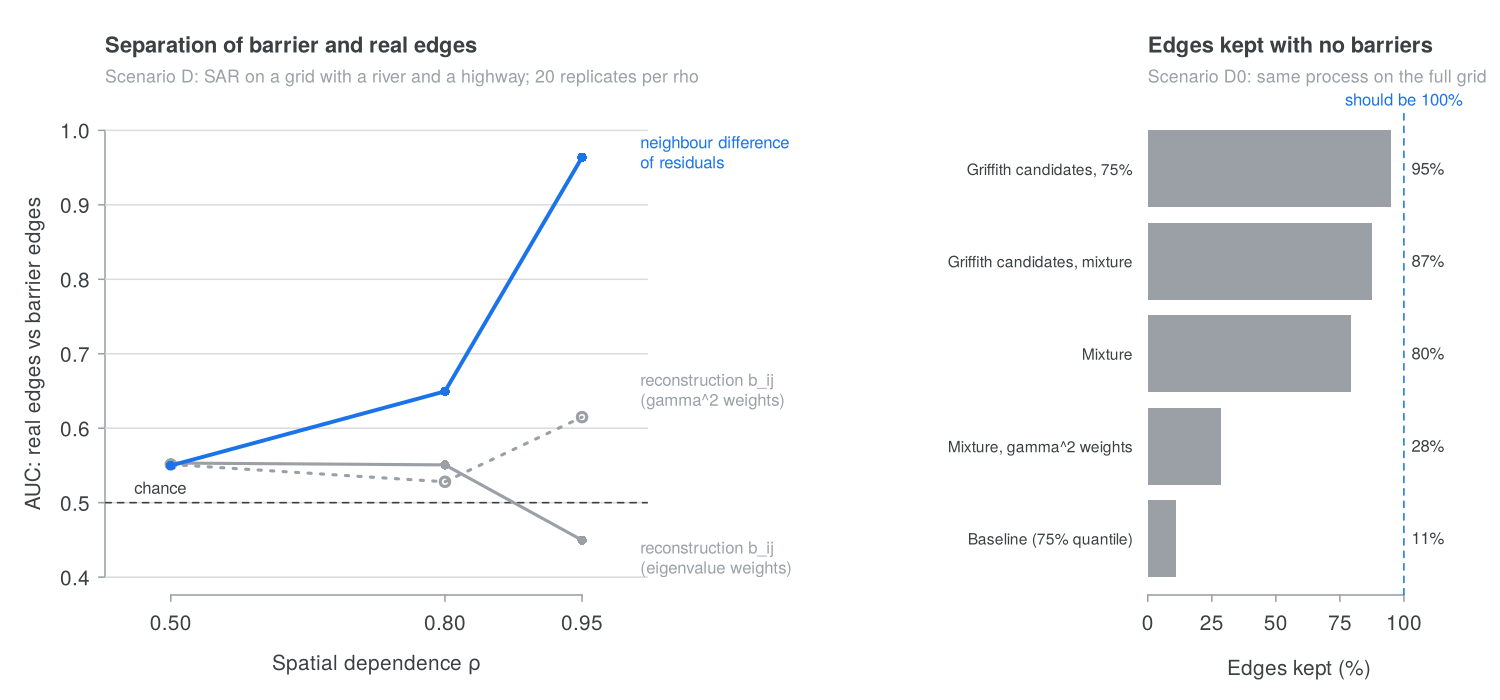
\includegraphics[width=\textwidth]{fig3_latent_graph}
\caption{Left: AUC for separating real edges from barrier edges in scenario D (20 replicates per $\rho$). Right: share of edges kept in scenario D0 by variant of the procedure.}
\label{fig:app-graph}
\end{figure}

\subsection{Conclusion}
\label{app:rec-conclusion}

In these simulations, no rounding rule increased the highest precision obtained without rounding by more than 0.01 (largest excess on the $20\times20$ grid; centrality among hot cells on the $40\times40$ grid). The reconstructed weights did not identify the edges removed by barriers, and most rounding rules removed most edges when no barrier was present. Ranking by centrality on the whole reconstructed graph selected cold cells in about half of the positions. The proposed procedure therefore uses the ESF step once, to estimate the spatial component $\hat f$ conditional on the covariates, and derives hot and cold zones from it on the contiguity graph $A$.
